
\documentclass{article} % For LaTeX2e
\usepackage{nips14submit_e,times}


% For figures
\usepackage{graphicx} % more modern
%\usepackage{epsfig} % less modern
\usepackage{caption}
\usepackage{subcaption}
\usepackage{amsmath,amsfonts,amsthm,amssymb}
\usepackage{listings}
\usepackage{tabularx}
\usepackage{multicol}
\usepackage{float}
\usepackage[protrusion=true,expansion=true]{microtype}
\usepackage{wrapfig}
\setlength{\emergencystretch}{3em}
\usepackage[numbers]{natbib}

\usepackage{multirow}

% For algorithms
\usepackage[algoruled,vlined,linesnumbered]{algorithm2e}
%\usepackage{algorithm}
\usepackage{algorithmic}

\usepackage{multicol}
\usepackage{comment}

% As of 2011, we use the hyperref package to produce hyperlinks in the
% resulting PDF.  If this breaks your system, please commend out the
% following usepackage line and replace \usepackage{icml2013} with
% \usepackage[nohyperref]{icml2013} above.
\usepackage{hyperref}

% Packages hyperref and algorithmic misbehave sometimes.  We can fix
% this with the following command.
\newcommand{\theHalgorithm}{\arabic{algorithm}}


\graphicspath{{figures/}}


\newcommand{\ie}{{\em i.e.,}~}
\newcommand{\eg}{{\em e.g.,}~}

\begingroup
    \makeatletter
    \@for\theoremstyle:=definition,remark,plain\do{%
        \expandafter\g@addto@macro\csname th@\theoremstyle\endcsname{%
            \addtolength\thm@preskip\parskip
            }%
        }
\endgroup
\newtheorem{dfn}{Definition}[section]
\newtheorem{thm}{Theorem}[section]
\newtheorem{cor}[thm]{Corollary}
\newtheorem{lem}[thm]{Lemma}
\newtheorem{prop}[thm]{Proposition}
\newtheorem{exmp}[thm]{Example}
\newtheorem{claim}{Claim}

\floatstyle{ruled}
\newfloat{program}{thp}{lop}
\floatname{program}{Program}

\newenvironment{denseitemize}{
\begin{itemize}[topsep=2pt, partopsep=0pt, leftmargin=1.5em]
  \setlength{\itemsep}{4pt}
  \setlength{\parskip}{0pt}
  \setlength{\parsep}{0pt}
}{\end{itemize}}

\newenvironment{packed_enum}{
\begin{enumerate}
  \setlength{\itemsep}{4pt}
  \setlength{\parskip}{0pt}
  \setlength{\parsep}{0pt}
}{\end{enumerate}}




\lstdefinelanguage{scala}{
  morekeywords={abstract,case,catch,class,def,%
    do,else,extends,false,final,finally,%
    for,if,implicit,import,match,mixin,%
    new,null,object,override,package,%
    private,protected,requires,return,sealed,%
    super,this,throw,trait,true,try,%
    type,val,var,while,with,yield},
  otherkeywords={=>,<-,<\%,<:,>:,\#,@},
  sensitive=true,
  morecomment=[l]{//},
  morecomment=[n]{/*}{*/},
  morestring=[b]",
  morestring=[b]',
%  numbers=left,
  morestring=[b]"""
}



% Commenting system
\newcommand{\Comments}{1}
\newcommand{\note}[2]{\ifnum\Comments=1\textcolor{#1}{#2}\fi}
\newcommand{\taunghao}[1]{\note{red}{[XP: #1]}}
\newcommand{\joey}[1]{\note{blue}{[JG: #1]}}
\newcommand{\stef}[1]{\note{green}{[SJ: #1]}}
\newcommand{\tb}[1]{\note{cyan}{[TB: #1]}}

\newcommand{\argmin}{\operatornamewithlimits{argmin}}






%% ---------------------------------------------------------
%% Terminology
\newcommand{\term}[1]{\textbf{#1}}


%% ---------------------------------------------------------
%% Citation/Reference commands
\newcommand{\citecf}[1]{(\cf, \cite{#1})}
\newcommand{\tableref}[1]{Table~\ref{#1}}
\newcommand{\figref}[1]{Figure~\ref{#1}}
\newcommand{\listref}[1]{Listing~\ref{#1}}

\newcommand{\eqnref}[1]{Eq.~(\ref{#1})}
\newcommand{\secref}[1]{Section~\ref{#1}}
\newcommand{\chapref}[1]{Chapter~\ref{#1}}

\newcommand{\dfnref}[1]{Definition~\ref{#1}}
\newcommand{\thmref}[1]{Theorem~\ref{#1}}
\newcommand{\propref}[1]{Prop.~\ref{#1}}
\newcommand{\lemref}[1]{Lemma~\ref{#1}}
\newcommand{\exmpref}[1]{Example~\ref{#1}}
\newcommand{\corref}[1]{Corollary~\ref{#1}}
\newcommand{\algref}[1]{Alg.~\ref{#1}}
\newcommand{\procref}[1]{Proc.~\ref{#1}}
\newcommand{\alglineref}[1]{Line~\ref{#1}}
\newcommand{\probref}[1]{Problem~(\ref{#1})}
\newcommand{\appendref}[1]{Appendix~\ref{#1}}

%% ---------------------------------------------------------
%% Basic Math
\newcommand{\abs}[1]{\left|#1\right|}
\newcommand{\ceil}[1]{\left\lceil #1 \right\rceil}
\newcommand{\floor}[1]{\left\lfloor #1 \right\rfloor}


%% ---------------------------------------------------------
%% special math functions
\newcommand{\polylog}[2]{\,\mathbf{Li}_{#1}\left( #2 \right)}
\newcommand{\harmonic}[2]{\,\mathbf{h}_{#1}\left( #2 \right)}

%% ---------------------------------------------------------
%% Norms
\newcommand{\Lone}{L_{1}}
\newcommand{\Linf}{L_{\infty}}
\newcommand{\LInfNorm}[1]{\left|\left| #1 \right|\right|_{\infty}}
\newcommand{\LOneNorm}[1]{\left|\left| #1 \right|\right|_1}



%% ---------------------------------------------------------
%% Probability notation
\newcommand{\given}{\,|\,}
\newcommand{\stdist}[1]{\mathbf{\pi} \left( #1 \right) }
\newcommand{\Prb}[1]{\mathbf{P} \left( #1 \right) }
\newcommand{\PrbEst}[1]{\mathbf{\tilde{P}} \left( #1 \right) }
\newcommand{\Ent}[1]{\mathbf{H} \left( #1 \right) }
\newcommand{\PiPrb}[1]{\Prb{ #1 } }
\newcommand{\Kern}[1]{K \left( #1 \right) }
\newcommand{\Ex}[1]{\mathbf{E} \left[ #1 \right] }
\newcommand{\Exwrt}[2]{\mathbf{E}_{#1} \left[ #2 \right] }
\newcommand{\Variance}[1]{\mathbf{Var} \left[ #1 \right] }
\newcommand{\Ind}[1]{\mathbf{1}\left[ #1 \right]}
\newcommand{\Bern}[1]{\text{Bern}( #1 ) }

%% ---------------------------------------------------------
%% Set notation
\newcommand{\reals}{\mathbb{R}}
\newcommand{\integers}{\mathbb{Z}}
\newcommand{\set}[1]{\left\{#1\right\}}
\newcommand{\vecspace}{\mathcal{V}}
\newcommand{\Union}{\bigcup}
\newcommand{\Inter}{\bigcap}
\newcommand{\union}{\cup}
\newcommand{\inter}{\cap}
\newcommand{\size}[1]{\left| #1 \right|}


%% ---------------------------------------------------------
%% Complexity
\newcommand{\BigO}[1]{O\hspace{-1pt}\left( #1 \right)}
\newcommand{\BigTheta}[1]{\Theta \left( #1 \right)}
\newcommand{\BigOmega}[1]{\Omega \left( #1 \right)}





%% ---------------------------------------------------------
%% Algorithms
\SetKwFor{ParForAll}{for}{do in parallel}{end}
\SetKwFunction{Map}{Map}
\SetKwFunction{Reduce}{Reduce}

\SetKwInput{Input}{Input}
\SetKwInput{Output}{Output}
\SetKwInput{SideEffect}{SideEffect}
\SetKwInput{Define}{Define}
\SetKwInput{Global}{Global}
\SetKwFor{DoWithProbability}{with probability}{}{}
\SetKwFunction{DPMeansOp}{DPMeansOp}
\SetKwFunction{DPValidate}{DPValidate}
\SetKwFunction{OFLValidate}{OFLValidate}
\SetKwFunction{BPMeansOp}{BPMeansOp}
\SetKwFunction{BPValidate}{BPValidate}
\SetKwFunction{NewClusters}{AcceptedClusters}

\SetKw{WaitUntil}{wait until}

\SetKwFunction{Mean}{Mean}
\SetKwFunction{Ref}{Ref}


%% ---------------------------------------------------------
%% Paper specific notation

% All the data
\newcommand{\data}{\mathcal{D}}
% \datablock{machine}
\newcommand{\datablock}[1]{\data_{#1}}

\newcommand{\clusters}{\mathcal{C}}
\newcommand{\gclusters}{\hat\clusters}
\newcommand{\newclusters}{\tilde\clusters}
% local clusters \lclusters{machine}
\newcommand{\lclusters}[1]{\clusters_{#1}}

%\newcommand{\bregd}[2]{D_\phi\left(#1,#2\right)}
\newcommand{\bregd}[2]{\left\|#1-#2\right\|}


% for ofl analysis:
\newcommand{\CFL}{C^{\text{FL}}}
\newcommand{\muFL}{\mu^{\text{FL}}}


\title{Parallel Double Greedy Submodular Maximization}

\author{
Xinghao Pan$^1$ Joseph Gonzalez$^1$ Stefanie Jegelka$^1$ Joseph Bradley$^{1}$ Michael I. Jordan$^{1,2}$\\
$^1$Department of Electrical Engineering and Computer Science, and $^2$Department of Statistics\\
University of California, Berkeley\\
Berkeley, CA USA 94720\\
  \texttt{\{xinghao,jegonzal,stefje,tab,?\}@eecs.berkeley.edu} \\
}

% \address{University of California
% 465 Soda Hall, MC-1776
% Berkeley, CA 94720-1776}

\newcommand{\fix}{\marginpar{FIX}}
\newcommand{\new}{\marginpar{NEW}}


%\nipsfinalcopy

\begin{document}


\maketitle


\begin{abstract}
Bidirectional greedy is a sequential algorithm that does not scale well to problems of large scale.
We present 2 approaches to extend the bidirectional greedy algorithm to a parallel setting.
The first, `hogwild' approach emphasizes speed at the cost of worsening the approximation by an additive factor;
the second approach guarantees the same approximation bound by sacrificing concurrency.
\end{abstract}

\section{Introduction}
The bidirectional greedy algorithm \cite{buchbinder2012} gives an approximation of $E[F(A)] = 1/2 f(OPT)$, where $A$ is the algorithm output, and $OPT$ is an optimal solution.

The hogwild algorithm can give an approximation of $E[F(A)] = \frac{1}{2} F(OPT) - \frac{1}{4}\sum_iE[\rho_i]$, where $\rho_i$ is the maximum difference in the marginal gain that may result from not knowing the full information when deciding whether to include or exclude element $i$.

The OCC algorithm \taunghao{for the lack of a better name} guarantees an outcome that is equivalent to a sequential run of the bidirectional greedy algorithm.
Theoretical properties of the bidirectional greedy algorithm immediately translates to the OCC algorithm -- in particular, the OCC algorithm gives the same approximation factor of $1/$.
In contrast to the hogwild approach, OCC introduces more coordination and thus provides less concurrency.











\section{Submodular maximization}

The sequential bidirectional greedy \cite{buchbinder2012} algorithm monotonically grows $A^i$ and shrinks $B^i$.









\section{Approaches for parallel learning}

Two approaches that allow us to trade off speed with approximation guarantees.

\subsection{Coordination free}
Simply run everything in parallel.
Optimized for speed, but does not necessarily provide the correct answer.
Requires work to prove correctness.

\subsection{Concurrency control}
Ensures `serial equivalence' -- the outcome of the parallel algorithm is equivalent to some execution of the sequential algorithm.
Locally, threads take actions that are guaranteed to be safe (i.e. preserves serial equivalence), and forces additional coordination only when they are unable to execute their action safely.
Designed for correctness, but requires coordination that compromises speed.
Work is only required to demonstrate that coordination is limited.


\begin{figure}[h]
  \footnotesize
  \centering
  \begin{multicols}{2}
    \begin{minipage}{0.49\textwidth}
      \begin{algorithm}[H]
        \DontPrintSemicolon
        \caption{Serial submodular maximization}
        \label{alg:submax}
        %\Input{}
        $A^0 = \emptyset$, $B^0 = V$\;
        \For{$i = 1$ to $n$}{
          $\Delta_{+}(i) = F(A^{i-1}\cup i) - F(A^{i-1})$\;
          $\Delta_{-}(i) = F(B^{i-1}\backslash i) - F(B^{i-1})$\;
          Draw $u_i\sim Unif(0,1)$\;
          \If {$u_i<\frac{[\Delta_{+}(i)]_+}{[\Delta_{+}(i)]_+ + [\Delta_{-}(i)]_+}$}{
            $A^i := A^{i-1} \cup i$;\\
            $B^i := B^{i-1}$\;
          }\Else{
            $A^i := A^{i-1}$;\\
            $B^i := B^{i-1}\backslash i$\;
          }
        }
        %\Output{$A_n$}
      \end{algorithm}
      
      
      \begin{algorithm}[H]
        \DontPrintSemicolon
        \caption{Hogwild bidirectional greedy}
        \label{alg:hogwild}
        \lFor{$e\in V$}{$\hat{A}(e) = 0$, $\hat{B}(e) = 1$}\;
        \ParForAll{$p \in \set{1, \ldots, P}$}{
          \While{$\exists$ element to process}{
            $e = $ next element to process\;
            $\Delta_{+}^{\max}(e) = F(\hat{A}\cup e) - F(\hat{A})$\;\label{alg:hogwild:deltaadd}
            $\Delta_{-}^{\max}(e) = F(\hat{B}\backslash e) - F(\hat{B})$\;\label{alg:hogwild:deltarem}
            Draw $u_e\sim Unif(0,1)$\;\label{alg:hogwild:time}
            \If {$u_e<\frac{[\Delta_{+}^{\max}(e)]_+}{[\Delta_{+}^{\min}(e)]_+ + [\Delta_{-}^{\max}(e)]_+}$}{
              $\hat{A}(e) \leftarrow 1$\;\label{alg:hogwild:add}
            }\lElse{
              $\hat{B}(e) \leftarrow 0$\;\label{alg:hogwild:rem}
            }
          }
        }
      \end{algorithm}


      \begin{algorithm}[H]
        \DontPrintSemicolon
        \caption{Hogwild for separable sums}
        \label{alg:hogwildsepsum}
        \lFor{$e\in V$}{$\hat{A}(e) = 0$}\;
        \lFor{$l = 1,\dots,L$}{$\hat\alpha_l = 0$, $\hat\beta_l = \sum_{e\in S_l}w_l(e)$}\;
        \ParForAll{$p \in \set{1, \ldots, P}$}{
          \While{$\exists$ element to process}{
            $e = $ next element to process\;
            $\Delta_+^{\max}(e) = -\lambda v(e) + \sum_{S_l\ni e} g(\hat\alpha_l + w_l(e)) - g(\hat\alpha_l)$\;
            $\Delta_-^{\max}(e) = +\lambda v(e) + \sum_{S_l\ni e} g(\hat\beta_l   - w_l(e)) - g(\hat\beta_l)$\;
            Draw $u_e\sim Unif(0,1)$\;
            \If {$u_e<\frac{[\Delta_{+}^{\max}(e)]_+}{[\Delta_{+}^{\min}(e)]_+ + [\Delta_{-}^{\max}(e)]_+}$}{
              $\hat{A}(e) \leftarrow 1$\;
              \lFor{$l: e \in S_l$}{
                $\hat\alpha_l \leftarrow \hat\alpha_l + w_l(e)$
              }
            }\lElse{
              \lFor{$l: e \in S_l$}{
                $\hat\beta_l \leftarrow \hat\beta_l - w_l(e)$
              }
            }
          }
        }
      \end{algorithm}
      
    \end{minipage}

    \begin{minipage}{0.49\textwidth}
\begin{algorithm}[H]
\DontPrintSemicolon
\caption{OCC bidirectional greedy}
\label{alg:occ}
\lFor{$e\in V$}{$\hat{A}(e) = \tilde{A}(e) = 0$, $\hat{B}(e) = \tilde{B}(e) = 1$}\;
\lFor{$i = 1,\dots,|V|$}{result$(i) = 0$}\;
\lFor{$i = 1,\dots,|V|$}{processed$(i) = false$}\;
$\iota = 0$\;
\ParForAll{$p \in \set{1, \ldots, P}$}{
  \While{$\exists$ element to process}{
    $e = $ next element to process\;
    $\tilde{A}(e) \leftarrow 1$\;
    $\tilde{B}(e) \leftarrow 0$\;
    $i = \iota$; $\iota \leftarrow \iota + 1$\;\label{alg:occ:time}
    $\Delta_+^{\min}(e) = F(\tilde{A} \cup e) - F(\tilde{A})$\;
    $\Delta_+^{\max}(e) = F(\hat{A}   \cup e) - F(\hat{A})$\;
    $\Delta_-^{\min}(e) = F(\tilde{B} \backslash e) - F(\tilde{B})$\;
    $\Delta_-^{\max}(e) = F(\hat{B}   \backslash e) - F(\hat{B})$\;
    Draw $u_e \sim Unif(0,1)$\;
    \If {$u_e < \frac{[\Delta_+^{\min}(e)]_+}{[\Delta_+^{\min}(e)]_+ + [\Delta_-^{\max}(e)]_+}$}{
      result$(i) \leftarrow 1$\;
    }\ElseIf {$u_e > \frac{[\Delta_+^{\max}(e)]_+}{[\Delta_+^{\max}(e)]_+ + [\Delta_-^{\min}(e)]_+}$}{
      result$(i) \leftarrow -1$\;
    }
    \WaitUntil $\forall j<i$, result$(j) \neq 0$\;
    \lIf {result$(i) = 0$}{validate($p$, $e$, $i$)}\;
    \If {result$(i) = 1$}{
      $\hat{A}(e)   \leftarrow 1$\;
      $\tilde{B}(e) \leftarrow 1$\;
    }\Else{
      $\tilde{A}(e) \leftarrow 0$\;
      $\hat{B}(e)   \leftarrow 0$\;
    }
    processed$(i) = true$\;
  }
}
\end{algorithm}

\begin{algorithm}[H]
\DontPrintSemicolon
\caption{validate($p$, $e$, $i$)}
\label{alg:occvalidate}
  \WaitUntil $\forall j < i$, processed$(j) = true$\;
  $\Delta_+(e) = F(\hat{A} \cup e) - F(\hat{A})$\;
  $\Delta_-(e) = F(\hat{B} \backslash e) - F(\hat{B})$\;
  \lIf {$u_e < \frac{[\Delta_+(e)]_+}{[\Delta_+(e)]_+ + [\Delta_-(e)]_+}$}{
    result$(i) \leftarrow 1$\;
  }\lElse{
    result$(i) \leftarrow -1$\;
  }
\end{algorithm}


  \label{fig:submax}
    \end{minipage}
    
    
    
  \end{multicols}
\end{figure}








\section{Hogwild for arbitrary submodular $F$}
Algorithm \ref{alg:hogwild} is the hogwild parallel bidirectional greedy unconstrained submodular maximization algorithm.
We associate with each element $e$ a time $T_e$ at which Algorithm \ref{alg:hogwild} line \ref{alg:hogwild:time} is executed, and order the elements according to the times $T_e$.
Let $\iota(e)$ be the position of $e$ in this ordering.
This total ordering on elements also allows us to define sets $A^i$, $B^i$ corresponding to that obtained by the serial algorithm;
specifically, $A^i = \{e' : e' \in A, \iota(e') < i\}$ and $B^i = A^i \cup \{e': \iota(e') \geq i\}$.

Note that in Algorithm \ref{alg:hogwild}, lines \ref{alg:hogwild:deltaadd} and \ref{alg:hogwild:deltarem} may be executed in parallel with lines \ref{alg:hogwild:add} and \ref{alg:hogwild:rem}.
Hence, $\Delta_+^{\max}(e)$ and $\Delta_-^{\max}(e)$ (lines \ref{alg:hogwild:deltaadd} and \ref{alg:hogwild:deltarem}) may be computed with different values of $\hat{A}(e')$.
We denote by $\hat{A}_e$ and $\hat{B}_e$ respectively the vectors of $\hat{A}$ and $\hat{B}$ that are used in the computation of $\Delta_+^{\max}(e)$ and $\Delta_-^{\max}(e)$.

\begin{lem}\label{lem:set_bound} For any $e\in V$, $\hat{A}_e \subseteq A^{\iota(e)-1}$, $\hat{B}_e \supseteq B^{\iota(e)-1}$.
\end{lem}
\begin{proof}
Consider any element $e'\in V$.
If $e'\in \hat{A}_e$, it must be the case that the algorithm set $\hat{A}(e')$ to 1 (line \ref{alg:hogwild:add}) before $T_e$, which implies $\iota(e') < \iota(e)$, and hence $e' \in A^{\iota(e)-1}$.
So $\hat{A}_e \subseteq A^{\iota(e)-1}$.

Similarly, if $e'\not\in \hat{B}_e$, then the algorithm set $\hat{B}(e')$ to 0 (line \ref{alg:hogwild:rem}) before $T_e$, so $\iota(e') < \iota(e)$.
Also, $e'\not\in A$ because the execution of line \ref{alg:hogwild:rem} excludes the execution of line \ref{alg:hogwild:add}.
Therefore, $e'\not\in A^{\iota(e)-1}$, and $e'\not\in B^{\iota(e)-1}$.
So $\hat{B}_e \subseteq B^{\iota(e)-1}$.
\end{proof}

It's easy to see that
\begin{align*}
  \Delta_{+}       (e) &= F(A^{\iota(e)-1}\cup i) - F(A^{\iota(e)-1}),
& \Delta_{-}       (e) &= F(B^{\iota(e)-1}\backslash e) - F(B^{\iota(e)-1})\\
  \Delta_{+}^{\max}(e) &= F(\hat{A}_e\cup e) - F(\hat{A}_e),
& \Delta_{-}^{\max}(e) &= F(\hat{B}_e\backslash e) - F(\hat{B}_e).
\end{align*}

\begin{cor}\label{cor:delta_bound}
Submodularity of $F$ implies that
\begin{align*}
  \Delta_{+}(e) &\quad\leq\quad \Delta_{+}^{\max}(e),
& \Delta_{-}(e) &\quad\leq\quad \Delta_{-}^{\max}(e).
\end{align*}
\end{cor}

\subsection{Hogwild for separable sums $F$}
For some functions $F$, we can maintain sketches / statistics to aid the computation of $\Delta_+^{\max}$, $\Delta_-^{\max}$, and obtain the bounds given in Corollary \ref{cor:delta_bound}.
In particular, we consider functions of the form
\begin{align*}
F(X) = \sum_{l=1}^L g\left(\sum_{i\in X\cup S_l} w_l(i)\right) - \lambda\sum_{i\in X} v(i),
\end{align*}
where $S_l \subseteq V$ are (possibly overlapping) groups of elements in the ground set, $g$ is a non-decreasing concave scalar function, and $w_l(i)$ and $v(i)$ are non-negative scalar weights.
It is easy to see that
\begin{align*}
F(X \cup e) - F(X) = \sum_{l: e\in S_l} \left[g\left(w_l(e) + \sum_{i\in X\cup S_l} w_l(i)\right) - g\left(\sum_{i\in X\cup S_l} w_l(i)\right)\right] - \lambda v(e).
\end{align*}
Define
\begin{align*}
  \hat\alpha_l              &= \sum_{j\in \hat{A}\cup S_l} w_l(j),
& \hat\alpha_{l,e}          &= \sum_{j\in \hat{A}_e\cup S_l} w_l(j),
& \alpha_l^{\iota(e)-1} &= \sum_{j\in A^{\iota(e)-1}\cup S_l} w_l(j).\\
  \hat\beta_l              &= \sum_{j\in \hat{B}\cup S_l} w_l(j),
& \hat\beta_{l,e}          &= \sum_{j\in \hat{B}_e\cup S_l} w_l(j),
& \beta_l^{\iota(e)-1} &= \sum_{j\in B^{\iota(e)-1}\cup S_l} w_l(j).
\end{align*}
We can update $\hat\alpha_l$ and $\hat\beta_l$ according to Algorithm \ref{alg:hogwildsepsum}.
Following arguments analogous to that of Lemma \ref{lem:set_bound}, we can show the following:

\begin{lem} For each $l$ and $e\in V$, $\hat\alpha_{l,e} \leq \alpha_l^{\iota(e)-1}$ and $\hat\beta_{l,e} \geq \beta_l^{\iota(e)-1}$.
\end{lem}

\begin{cor} Concavity of $g$ implies
\begin{align*}
\Delta_+^{\max}(e)
&= \sum_{l:e\in S_l} \left[g(\hat\alpha_{l,e} + w_l(e)) - g(\hat\alpha_{l,e})\right] - \lambda v(e)\\
&\geq \sum_{l:e\in S_l} \left[g(\hat\alpha_l^{\iota(e)-1} + w_l(e)) - g(\hat\alpha_l^{\iota(e)-1})\right] - \lambda v(e)
&= \Delta_+(e),\\
\Delta_-^{\max}(e)
&= \sum_{l:e\in S_l} \left[g(\hat\beta_{l,e} - w_l(e)) - g(\hat\beta_{l,e})\right] + \lambda v(e)\\
&\geq \sum_{l:e\in S_l} \left[g(\hat\beta_l^{\iota(e)-1} - w_l(e)) - g(\hat\beta_l^{\iota(e)-1})\right] + \lambda v(e)
&= \Delta_-(e),
\end{align*}
\end{cor}








\section{Concurrency control}

Algorithm \ref{alg:occ} is the OCC bidirectional greedy algorithm.
Unlike the hogwild algorithm, the OCC algorithm ensures serial equivalence by maintaining four sets $\hat{A}$, $\tilde{A}$, $\hat{B}$, $\tilde{B}$, which serve as upper and lower bounds on $A$ and $B$.
Each thread can determine locally if a decision to include / exclude an element can be taken safely.
Otherwise, the validation process (Algorithm \ref{alg:occvalidate}) waits until it is certain about $A$, $B$ before proceeding.

The serialization order is given by $\iota(e)$, which is the value of $\iota$ at line \ref{alg:occ:time} of Algorithm \ref{alg:occ}.
We will show that the outcome of Algorithm \ref{alg:occ} is equivalent to the sequential algorithm executed with ordering given by $\iota$.

\begin{lem} $\hat{A}_e \subseteq A^{\iota(e)-1} \subseteq \tilde{A}_e \backslash e$, and $\hat{B}_e \supseteq B^{\iota(e)-1} \supseteq \tilde{B}_e \backslash e$.
\end{lem}
\begin{proof}
There are 4 parts to this proof.
\begin{enumerate}
\item $e' \in \hat{A}_e \implies e' \in A^{\iota(e)-1}$.
\item $e' \in A^{\iota(e)-1} \implies e' \in\tilde{A}_e \backslash e$.
\item $e' \not\in \hat{B}_e \implies e' \not\in B^{\iota(e)-1}$.
\item $e' \not\in B^{\iota(e)-1} \implies e' \not\in\tilde{B}_e \backslash e$.
\end{enumerate}
\end{proof}

We can compute
\begin{align*}
  \Delta_+^{\min}(e) &= F(\tilde{A}_e) - F(\tilde{A}_e \backslash e),
& \Delta_+^{\max}(e) &= F(\hat{A}_e \cup e) - F(\hat{A})\\
  \Delta_-^{\min}(e) &= F(\tilde{B}_e) - F(\tilde{B}_e \cup e),
& \Delta_-^{\max}(e) &= F(\hat{B}_e \backslash e) - F(\hat{B}).
\end{align*}

\begin{cor} By submodularity of $F$, $\Delta_+^{\min}(e) \leq \Delta_+(e) \leq \Delta_+^{\max}(e)$, and $\Delta_-^{\min}(e) \leq \Delta_-(e) \leq \Delta_-^{\max}(e)$.
\end{cor}

\subsection{Separable sums $F$}
We maintain $\tilde\alpha_l$, $\hat\alpha_l$, $\tilde\beta_l$, $\hat\beta_l$.
It can be shown that $\hat\alpha_{l,e} \leq \alpha^{\iota(e)-1} \leq \tilde\alpha_{l,e} - w_l(e)$ and $\hat\alpha_{l,e} \geq \beta^{\iota(e)-1} \geq \tilde\beta_{l,e} + w_l(e)$, which then allows us to compute our bounds for $\Delta$'s.

~











\section{Analysis of algorithms}

\subsection{Approximation of hogwild bidirectional greedy}
\begin{thm}\label{thm:randomapprox} Let $F$ be a non-negative (monotone or non-monotone) submodular function.
The hogwild bidirectional greedy algorithm solves the unconstrained problem $\max_{A\subset V} F(A)$ with approximation
\[
E[F(A)] \geq \frac{1}{2}F^* - \frac{1}{4}\sum_{i=1}^n E[\rho_i],
\]
where $A$ is the output of the algorithm, $F^*$ is the optimal value, and $\rho_i$ is a random variable such that $\rho_i \geq \Delta_+^{\max}(i) - \Delta_+(i)$ and $\rho_i \geq \Delta_-^{\max}(i) - \Delta_-(i)$.
\end{thm}

We prove the theorem in Appendix \ref{app:proofhogwild}.

\textbf{Assumption}

$F$ is submodular and non-negative.
We assume that we can bound
\begin{align*}
&\Delta_+^{\max} - \rho_i \leq \Delta_+ \leq \Delta_+^{\max} \leq \Delta_+ + \rho_i,&
&\Delta_-^{\max} - \rho_i \leq \Delta_- \leq \Delta_-^{\max} \leq \Delta_- + \rho_i
\end{align*}

This is possible, for example, by defining
\begin{align*}
\rho_i
&:= \max\{\Delta_+^{\max}(i) - \Delta_+(i), \Delta_-^{\max}(i) - \Delta_-(i)\}\\
&\leq \max_{S,T\subseteq V} \{[F(S\cup i) - F(S)] - [F(S \cup T \cup i) - F(S \cup T)]\}\\
&\leq F(i) - F(\emptyset) - F(V) + F(V\backslash i)\\
&\leq F(i)\left(1 - \frac{F(V) - F(V\backslash i)}{F(i)}\right)\\
&= F(i)\kappa_F
\end{align*}
where $S$ plays the role of $A^j$ and $T$ plays the role of $\{j+1,\dots, i-1\}$, and $\kappa_F$ is the total curvature of $F$.
Summing over $i$ then gives us $\sum_i \rho_i \leq \kappa_F\sum_i F(i)$.

\taunghao{Is there theory along these lines? Can we tighten this for non-monotone functions?}


\textbf{Example: max graph cut}

Assuming bounded delay of $\tau$ and edges with unit weight, we can bound $\sum_i E[\rho_i] \leq 2\tau\frac{\text{\#edges}}{2N}$
The approximation of the hogwild algorithm is then $E[F(A^n)] \geq = \frac{1}{2} F(OPT) - \tau\frac{\#\text{edges}}{2N}$.
In sparse graphs, the hogwild algorithm is off by a small additional term, which albeit grows linearly in $\tau$.



\textbf{Example: set cover}

\taunghao{For now, consider a toy problem, with (1) disjoint sets, (2) bounded delay, (3) $\lambda \leq 1$.}

Consider the simple set cover function,
$F(A) = \sum_{l=1}^L \min(1,|A\cap S_l|) - \lambda|A| = |\{l: A\cap S_l \neq\emptyset\}| - \lambda|A|$,
with $0 < \lambda \leq 1$.
We assume that there is some bounded delay $\tau$.
Suppose also the $S_l$'s form a partition, so each element $e$ belongs to exactly one set.
Then, $\sum_e E[\rho_e] \geq \tau + L(1-\lambda^\tau)$, which is linear in $\tau$ but independent of $N$.


\subsection{Correctness of OCC}
\begin{thm} OCC bidirectional greedy is serially equivalent to bidirectional greedy.
\end{thm}
\begin{proof}
Outline of proof: We need to show 2 things.
Firstly, that the sampling using $\Delta_+^{min}$, $\Delta_+^{max}$, $\Delta_-^{min}$, $\Delta_-^{max}$ is `safe', i.e. is equivalently to sampling using $\Delta_+$ and $\Delta_-$.
Secondly, that the validation process is correct -- specifically that when the validation is executed, it is in fact the case that $\hat{A} = A^{\iota(e)-1}$ and $\hat{B} = B^{\iota(e)-1}$.
\end{proof}



\subsection{Scalability of OCC}

We discuss the bound on the number of elements sent for validation in Appendix \ref{app:proofocc}

\textbf{Example: max graph cut}

The expected number of validated elements is upper bounded by $\tau \frac{2\#edges}{N}$.

\textbf{Example: set cover}

Under the same settings as for the hogwild analysis, the expected number of validated elements is upper bounded by $2\tau$.

















\section{Evaluation}

\subsection{Implementation}
Code in Java / Scala.

\begin{comment}
\subsection{Experiments, laptop}
Experiments run on laptop. Averaged over 10 iterations.

\begin{table}[ht]
\begin{tabular}{|c|c|c|c|c|c|c|c|}
\hline
\multirow{2}{*}{\# threads} & \multicolumn{3}{c|}{OCC} & \multicolumn{4}{c|}{Hogwild}\\
 & Runtime & Relative & \# validated & Runtime & Relative & $F(A)$ & \# diff from seq.\\\hline
Seq.	&3493	&2.54	&0.0	&3493	&1.23	&496595	&0.0\\\hline
1	&8872	&1.00	&0.0	&4289	&1.00	&496595	&0.0\\\hline
2	&5276	&1.68	&0.0	&2271	&1.89	&496595	&0.0\\\hline
3	&4112	&2.16	&0.7	&1693	&2.53	&496595	&2.5\\\hline
4	&3793	&2.34	&3.1	&1445	&2.97	&496595	&6.8\\\hline
5	&3361	&2.64	&4.9	&1305	&3.29	&496595	&11.4\\\hline
6	&3051	&2.91	&5.1	&1161	&3.69	&496594	&12.0\\\hline
\end{tabular}
\caption{\textbf{Set Cover:} 50,000 elements, covering 500,000 groups, in a random graph with edge probability of 0.002}
\end{table}


\begin{table}[ht]
\begin{tabular}{|c|c|c|c|c|c|c|c|}
\hline
\multirow{2}{*}{\# threads} & \multicolumn{3}{c|}{OCC} & \multicolumn{4}{c|}{Hogwild}\\
 & Runtime & Relative & \# validated & Runtime & Relative & $F(A)$ & \# diff from seq.\\\hline
Seq.	&1229	&1.03	&0.0	&1229	&0.97	&62662830	&0.0\\\hline
1	&1264	&1.00	&0.0	&1196	&1.00	&62662830	&0.0\\\hline
2	&821	&1.54	&0.2	&605	&1.98	&62662830	&0.0\\\hline
3	&602	&2.10	&0.4	&439	&2.72	&62662830	&0.0\\\hline
4	&528	&2.39	&1.3	&393	&3.04	&62662745	&6.3\\\hline
5	&507	&2.49	&1.8	&325	&3.68	&62662831	&1.4\\\hline
6	&421	&3.00	&1.4	&287	&4.17	&62662747	&5.7\\\hline
\end{tabular}
\caption{\textbf{Graph Cut:} 50,000 vertices, in a random graph with edge probability of 0.05}
\end{table}


Runtime is given in milliseconds.
`Relative' runtime refers to the runtime relative to that of using 1 thread.
Ideally, the runtime of the parallel algorithm should be lesser than the sequential algorithm, and have a relative runtime that scales linearly with the number of threads (e.g. running on 5 threads should have a relative runtime of 5).

Due to the effort needed for coordination and maintaining additional sets, the OCC algorithm is initially slower than the sequential algorithm, but quickly outperforms it as more threads are added.
We counted the number of elements that had to be validated, which required major coordination and slow down in the algorithm.
The number of validated elements increased with the number of threads (which explains the failure of OCC to scale less than linearly), but is still less than 1\% of the total number of elements when 5 threads are used.

We also verified the correctness of the OCC algorithm by comparing the output sets with the sequential algorithm executed under the same ordering of elements.

The hogwild algorithm has better scaling than OCC, since it requires almost no coordination.
We also measured the objective value $F(A)$ for hogwild.
For the set cover problem, hogwild performs just as well as the sequential algorithm, even though it does not provide exactly the same output set.
On the graph cut problem, the difference in the objective value is less than 0.01\%.
\end{comment}



\subsection{Experiments, synthetic}
\begin{figure}[ht]
  \centering
  \begin{tabular}{cc}
	  \begin{subfigure}[b]{0.5\textwidth}
	  	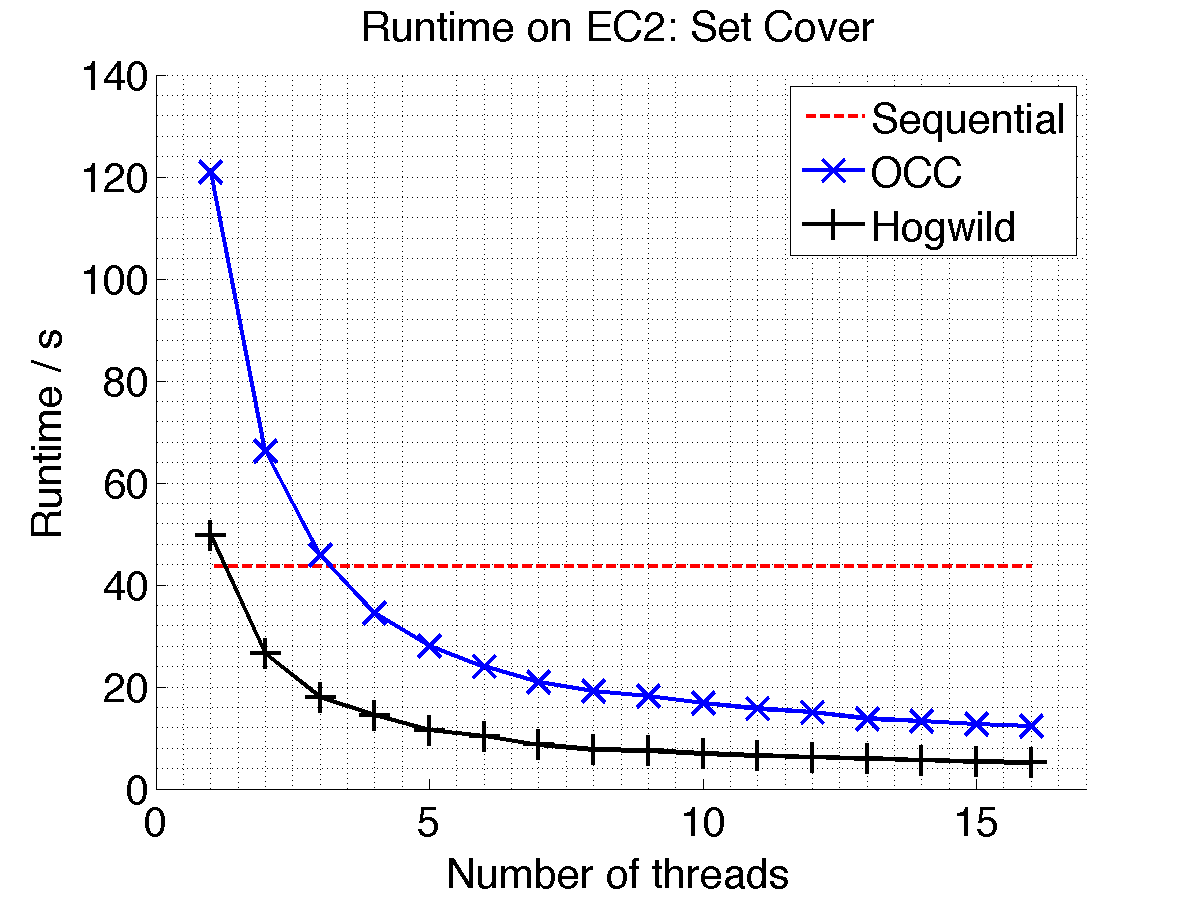
\includegraphics[width=200pt]{images/runtime_setcover_500000.png}
			\caption{Runtime, set cover}
			\label{fig:runtime_setcover}
	  \end{subfigure} &
	  \begin{subfigure}[b]{0.5\textwidth}
	  	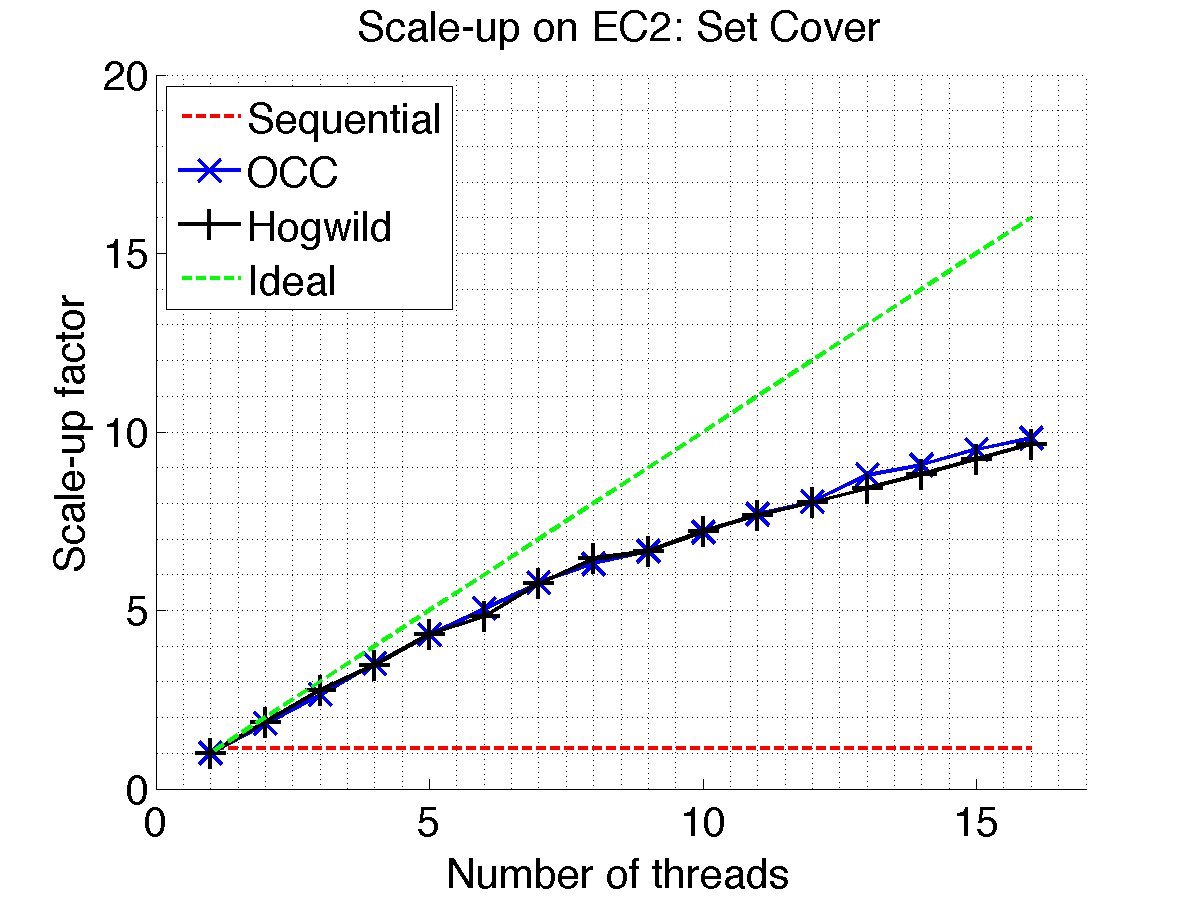
\includegraphics[width=200pt]{images/scaleup_setcover_500000.png}
			\caption{Scale-up, set cover}
			\label{fig:scale_setcover}
	  \end{subfigure} \\
	  \begin{subfigure}[b]{0.5\textwidth}
	  	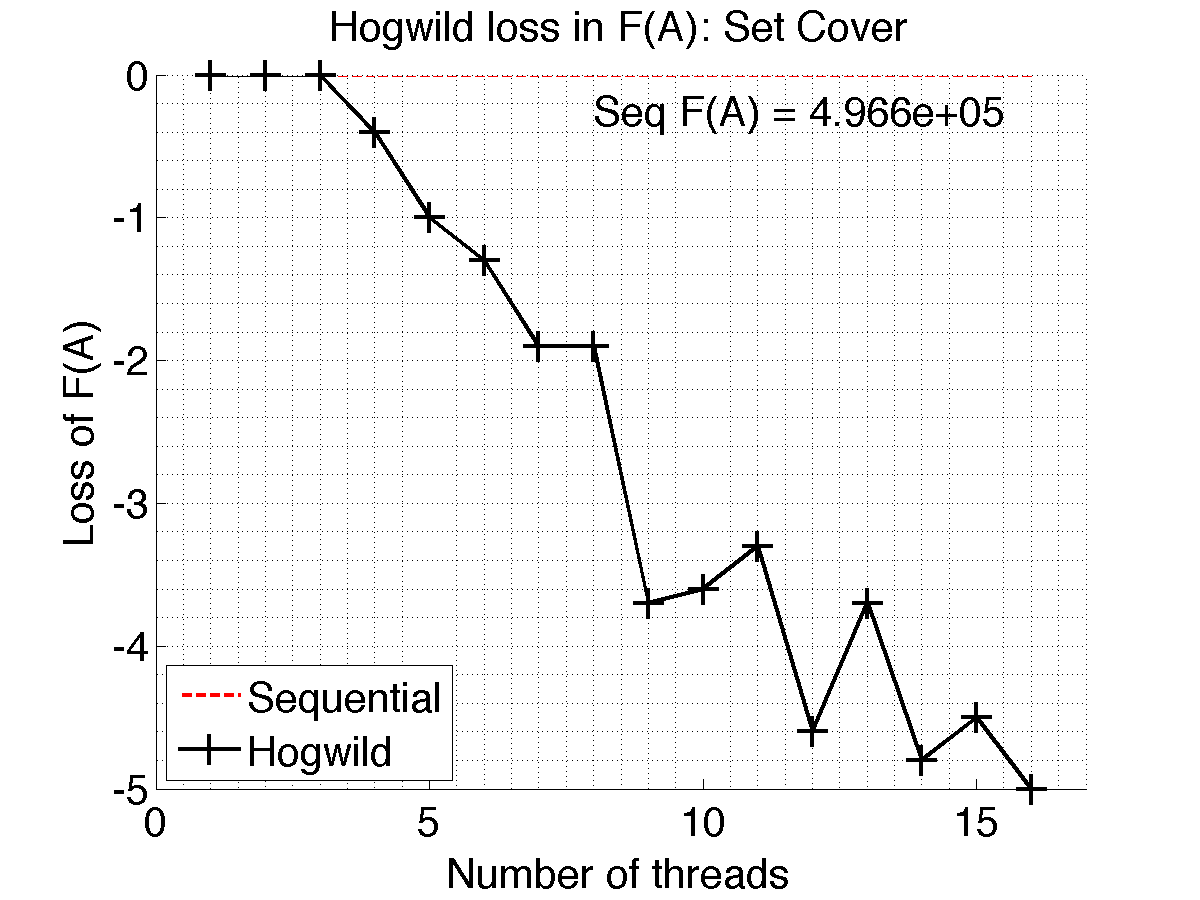
\includegraphics[width=200pt]{images/diffFA_Hogwild_setcover_500000.png}
			\caption{Hogwild diff $F(A)$, set cover}
			\label{fig:hogdiffFA_setcover}
	  \end{subfigure} &
	  \begin{subfigure}[b]{0.5\textwidth}
	  	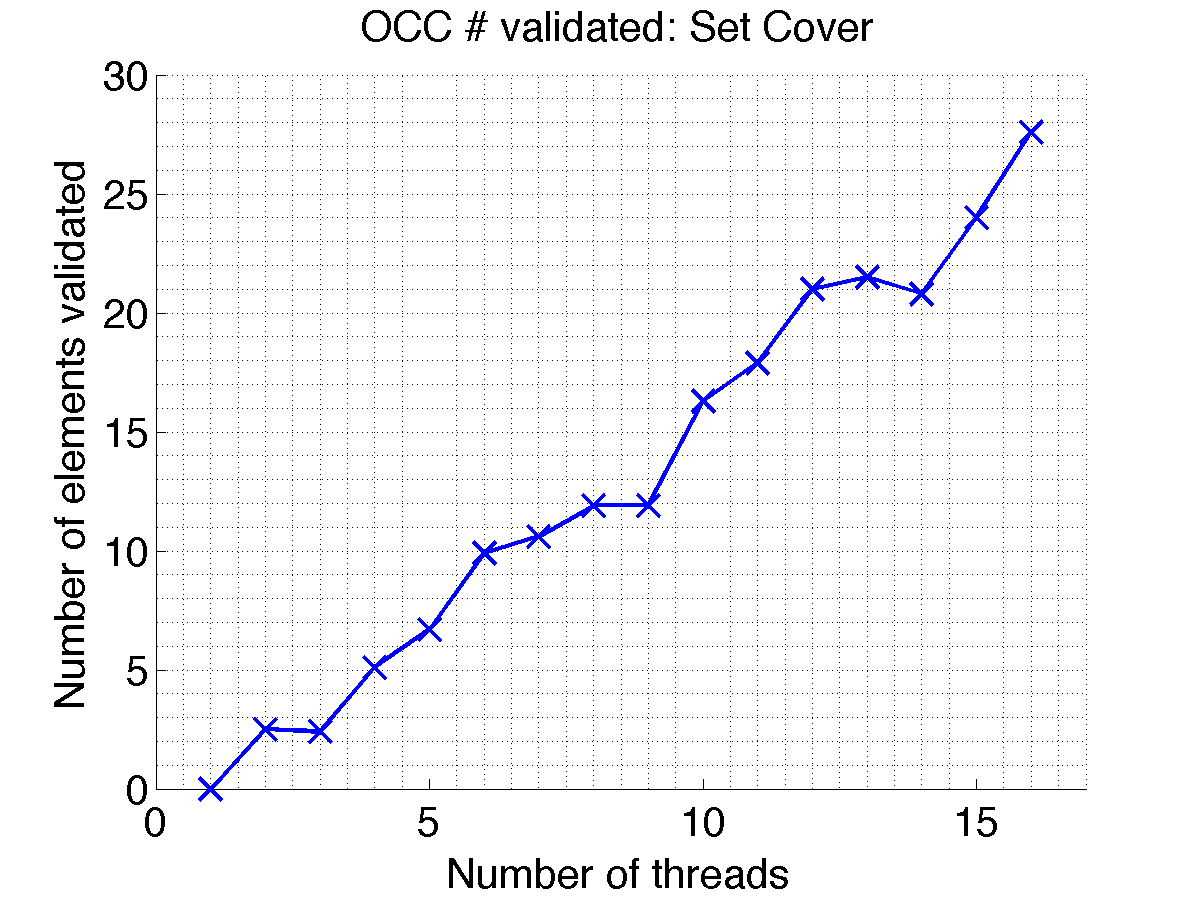
\includegraphics[width=200pt]{images/validated_OCC_setcover_500000.png}
			\caption{OCC \# validated, set cover}
			\label{fig:occsvalidated_setcover}
	  \end{subfigure} \\
	\end{tabular}
	\caption{\textbf{Synthetic data, Set Cover:} 500,000 elements, covering 500,000 groups, in a random graph with edge probability of 0.002}
\end{figure}

\begin{figure}[ht]
  \centering
  \begin{tabular}{cc}
	  \begin{subfigure}[b]{0.5\textwidth}
	  	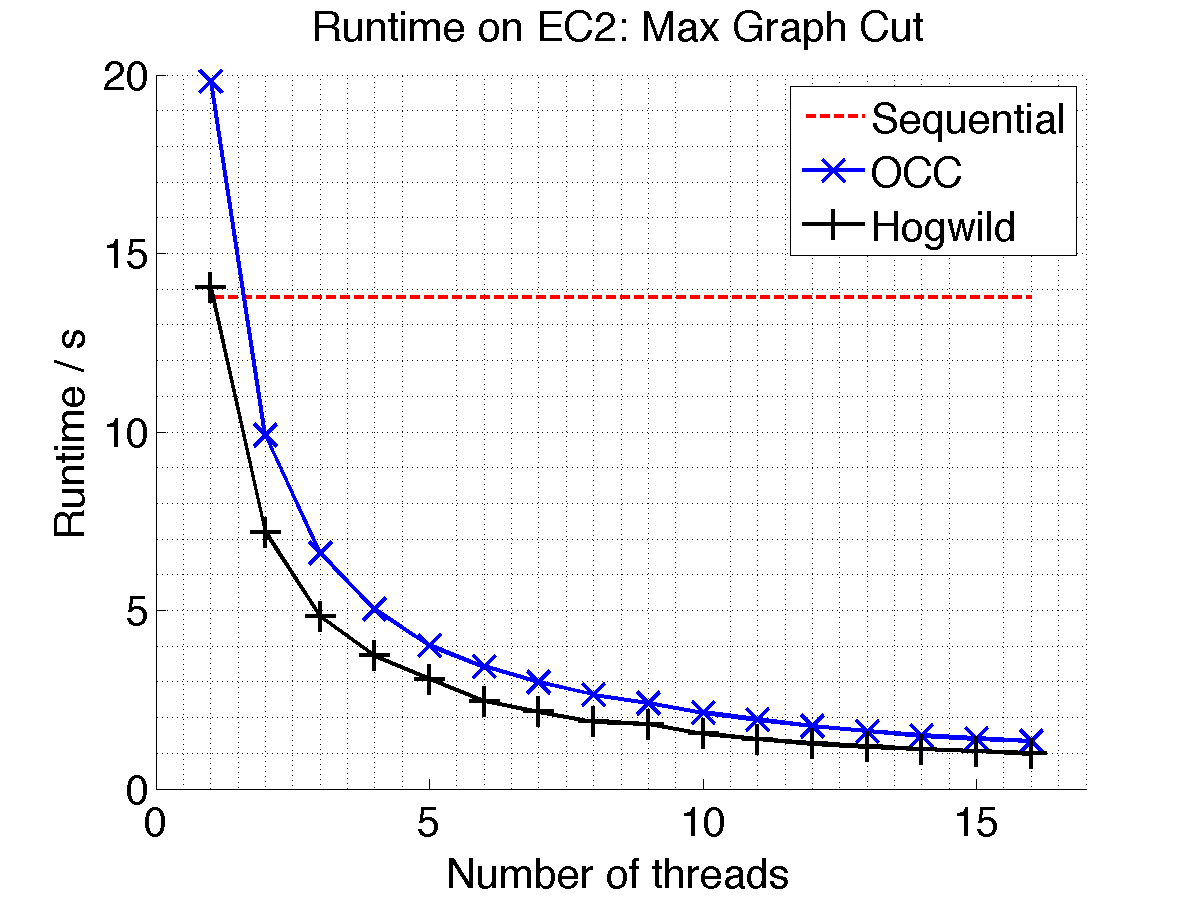
\includegraphics[width=200pt]{images/runtime_maxgraphcut_500000_2.png}
			\caption{Runtime, max graph cut}
			\label{fig:runtime_maxgraphcut}
	  \end{subfigure} &
	  \begin{subfigure}[b]{0.5\textwidth}
	  	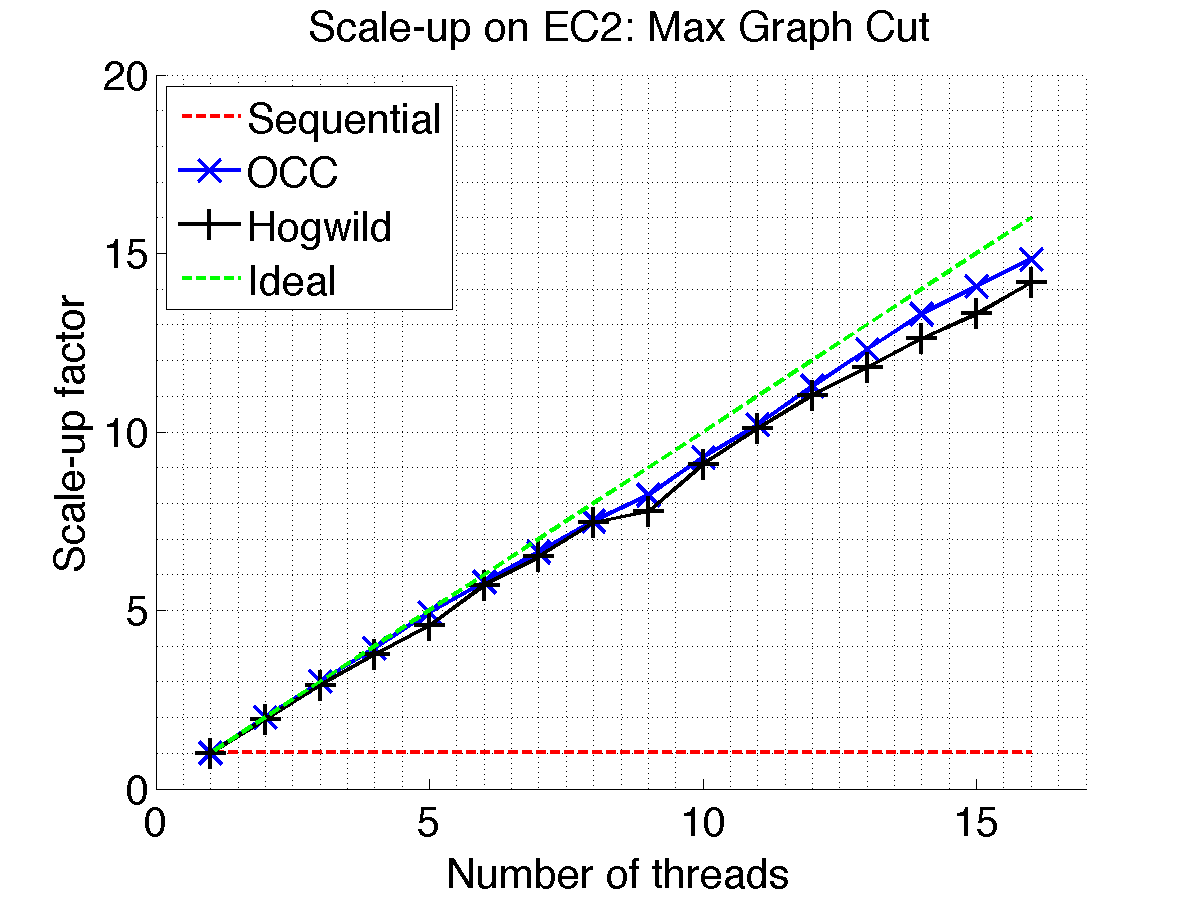
\includegraphics[width=200pt]{images/scaleup_maxgraphcut_500000_2.png}
			\caption{Scale-up, max graph cut}
			\label{fig:scale_maxgraphcut}
	  \end{subfigure} \\
	  \begin{subfigure}[b]{0.5\textwidth}
	  	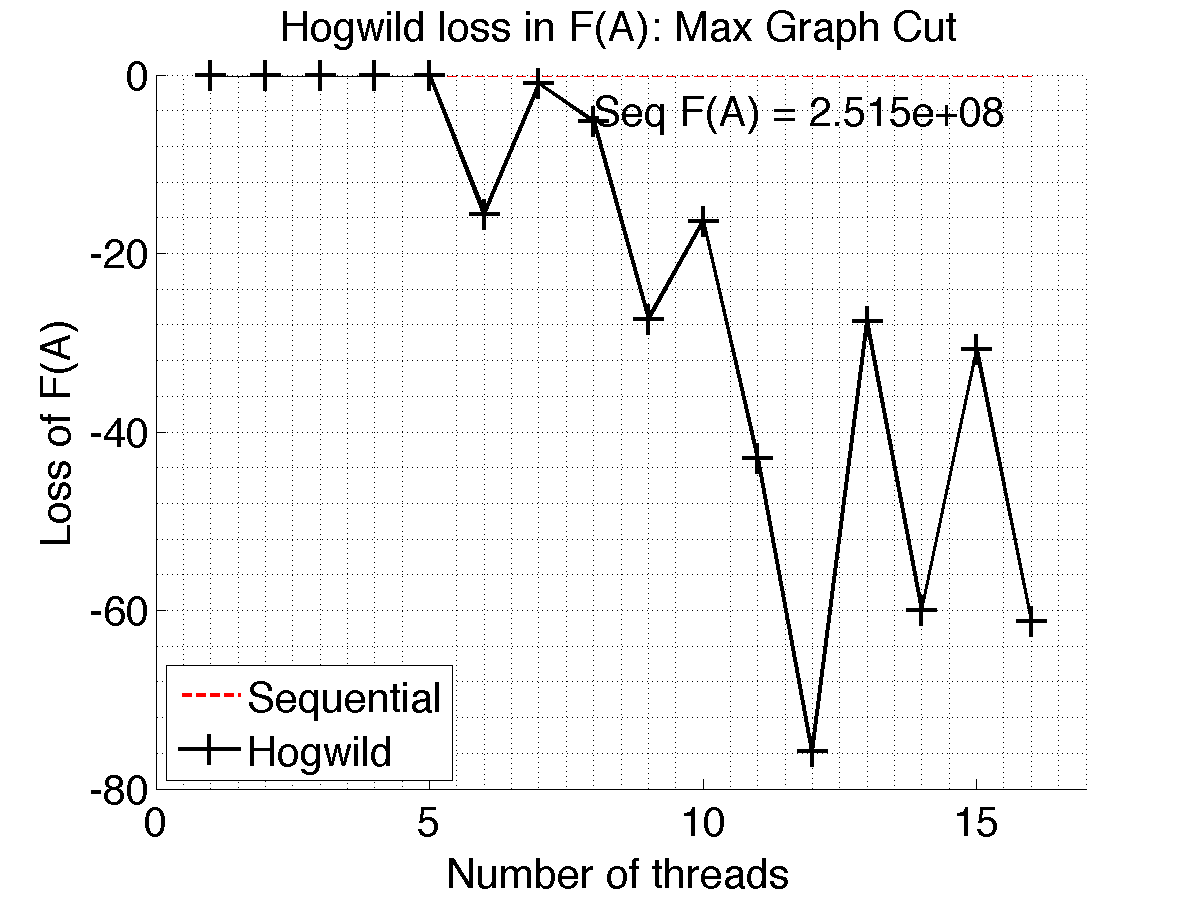
\includegraphics[width=200pt]{images/diffFA_Hogwild_maxgraphcut_500000_2.png}
			\caption{Hogwild diff $F(A)$, max graph cut}
			\label{fig:hogdiffFA_maxgraphcut}
	  \end{subfigure} &
	  \begin{subfigure}[b]{0.5\textwidth}
	  	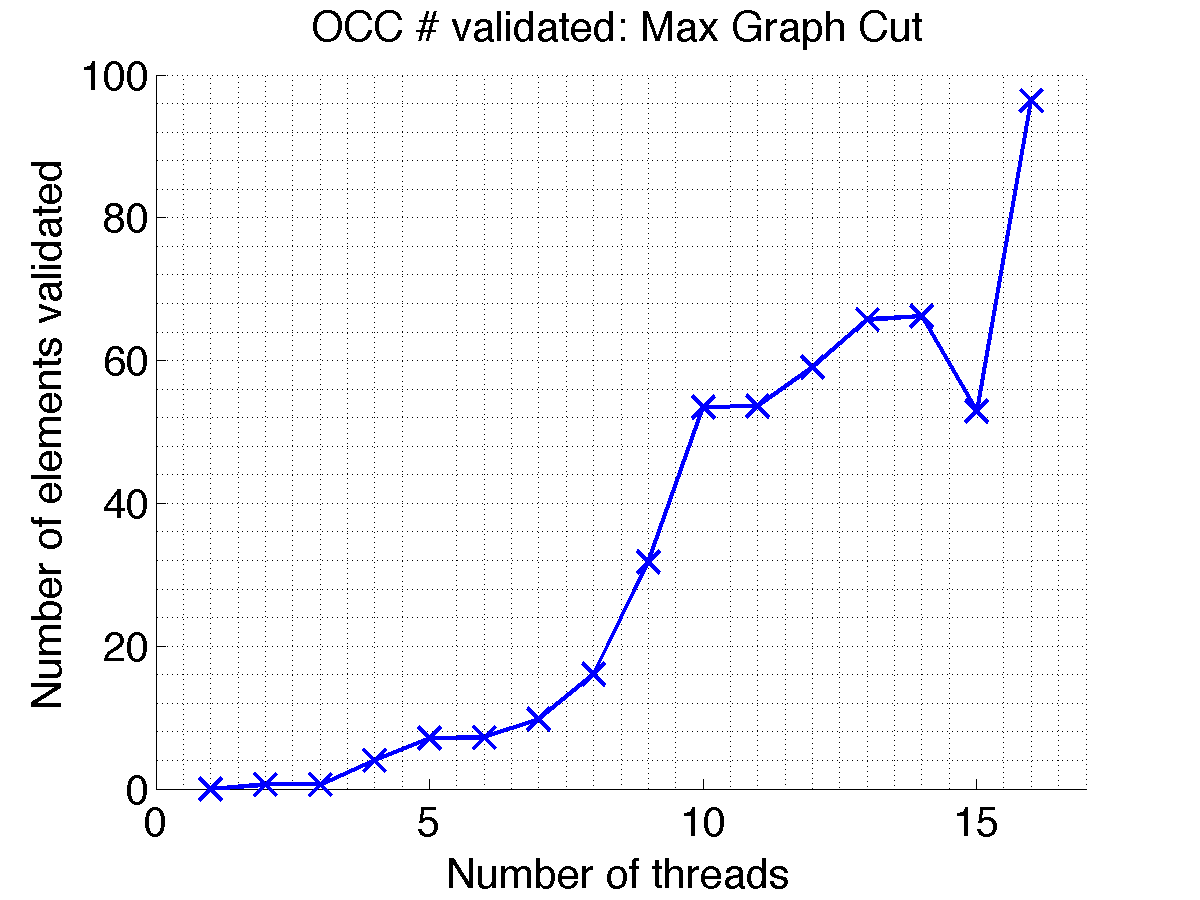
\includegraphics[width=200pt]{images/validated_OCC_maxgraphcut_500000_2.png}
			\caption{OCC \# validated, max graph cut}
			\label{fig:occsvalidated_maxgraphcut}
	  \end{subfigure} \\
	\end{tabular}
	\caption{\textbf{Synthetic data, Graph Cut:} 500,000 vertices, in a random graph with edge probability of 0.002}
\end{figure}

Experiments run on EC2, single cc2.8xlarge (32 vCPUs, 60.5GiB memory) machine.

Averaged over 10 iterations.




\subsection{Experiments, real graphs}
Experiments were run on the following real graphs.
Graphs were pre-processed to remove self-loops.
We found that vertices were typically indexed such that vertices close to each another in the graph were also close in their indices.
To reduce this dependency, we randomly permuted the ordering of vertices.

For the max graph cut problem, we removed directions on edges to obtain undirected graphs.
The set cover problem is reduced to a vertex cover on the directed graph.

\begin{table}[h]
\centering
\begin{tabular}{|c|c|c|c|}\hline
Graph & \# vertices & \# undirected edges & \# directed edges\\\hline\hline
Google & 875,713 & 2,359,034 & 4,563,235\\\hline
BerkStan & 685,230 & 3,860,581 & 7,600,595\\\hline
Live Journal & 3,997,962 & 33,099,465 & 68,475,391\\\hline
Orkut & 3,072,441 & 117,181,608 & 117,181,608\\\hline
Friendster\footnote{We used only a subset consisting of the first 8 million vertices so that we would not run into out-of-memory errors.} & 8,000,000 &  & 239,763,187\\\hline
\end{tabular}
\end{table}



\begin{figure}[ht]
  \centering
  \begin{tabular}{ccc}
	  \begin{subfigure}[b]{0.31\textwidth}
	  	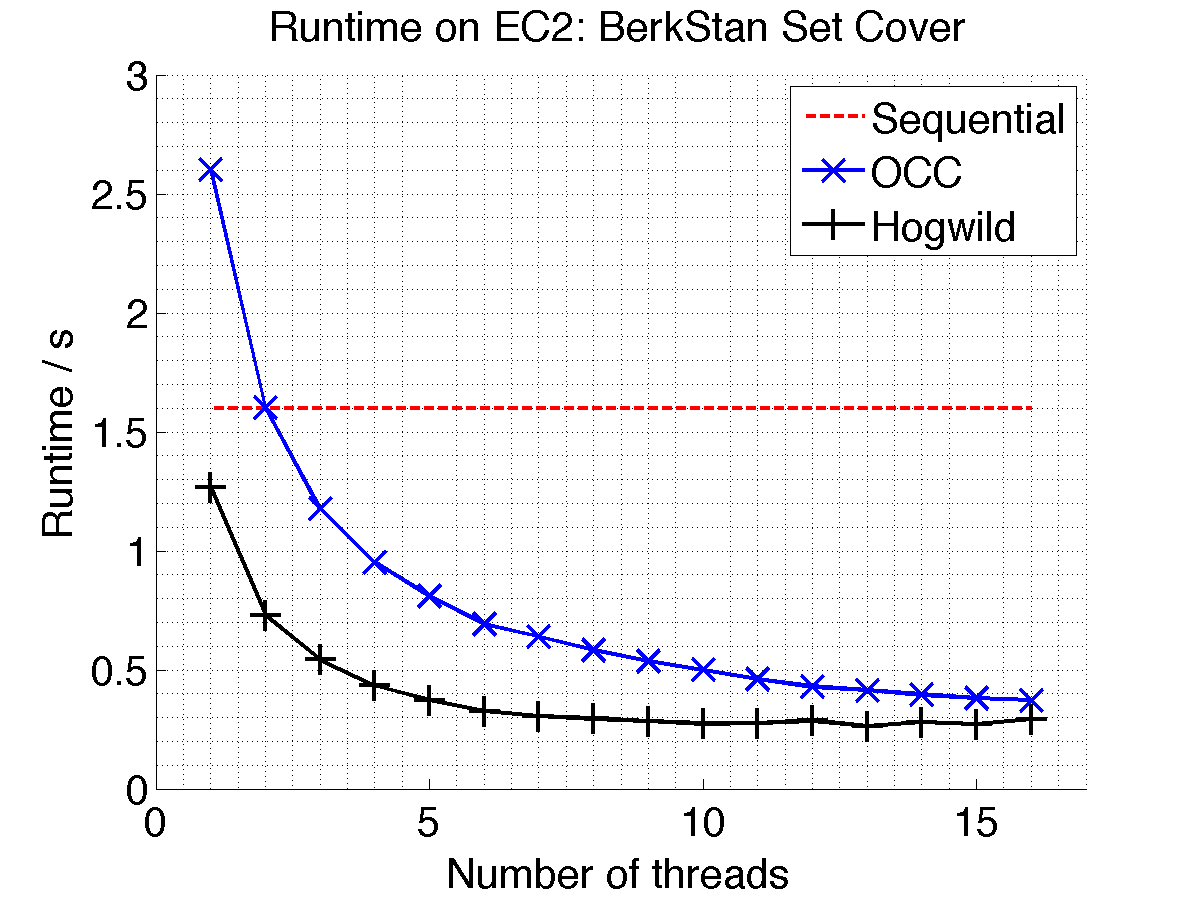
\includegraphics[width=150pt]{images/runtime_webberkstan_setcover.png}
			\caption{Runtime, BerkStan}
			\label{fig:runtime_webberkstan_setcover}
	  \end{subfigure} &
	  \begin{subfigure}[b]{0.31\textwidth}
	  	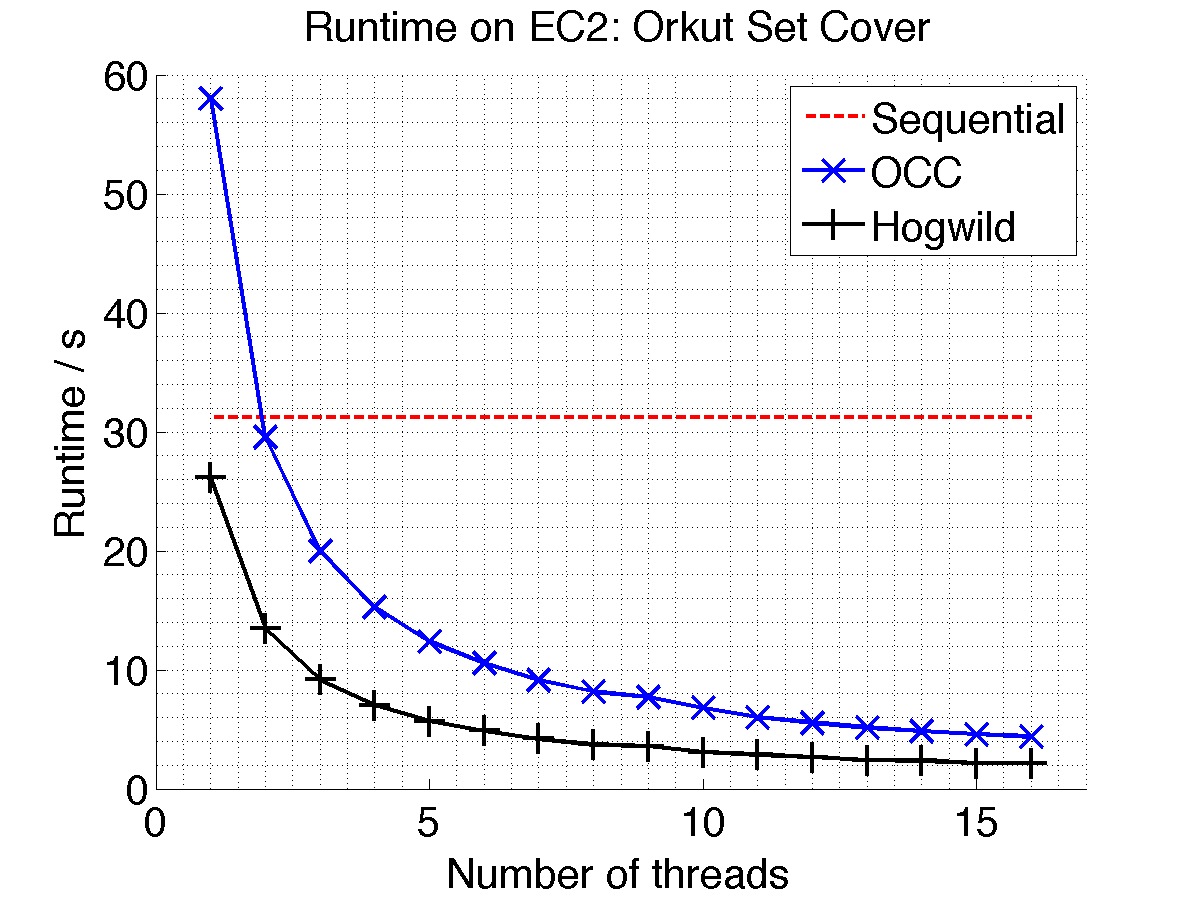
\includegraphics[width=150pt]{images/runtime_orkut_setcover.png}
			\caption{Runtime, Orkut}
			\label{fig:runtime_orkut_setcover}
	  \end{subfigure} &
	  \begin{subfigure}[b]{0.31\textwidth}
	  	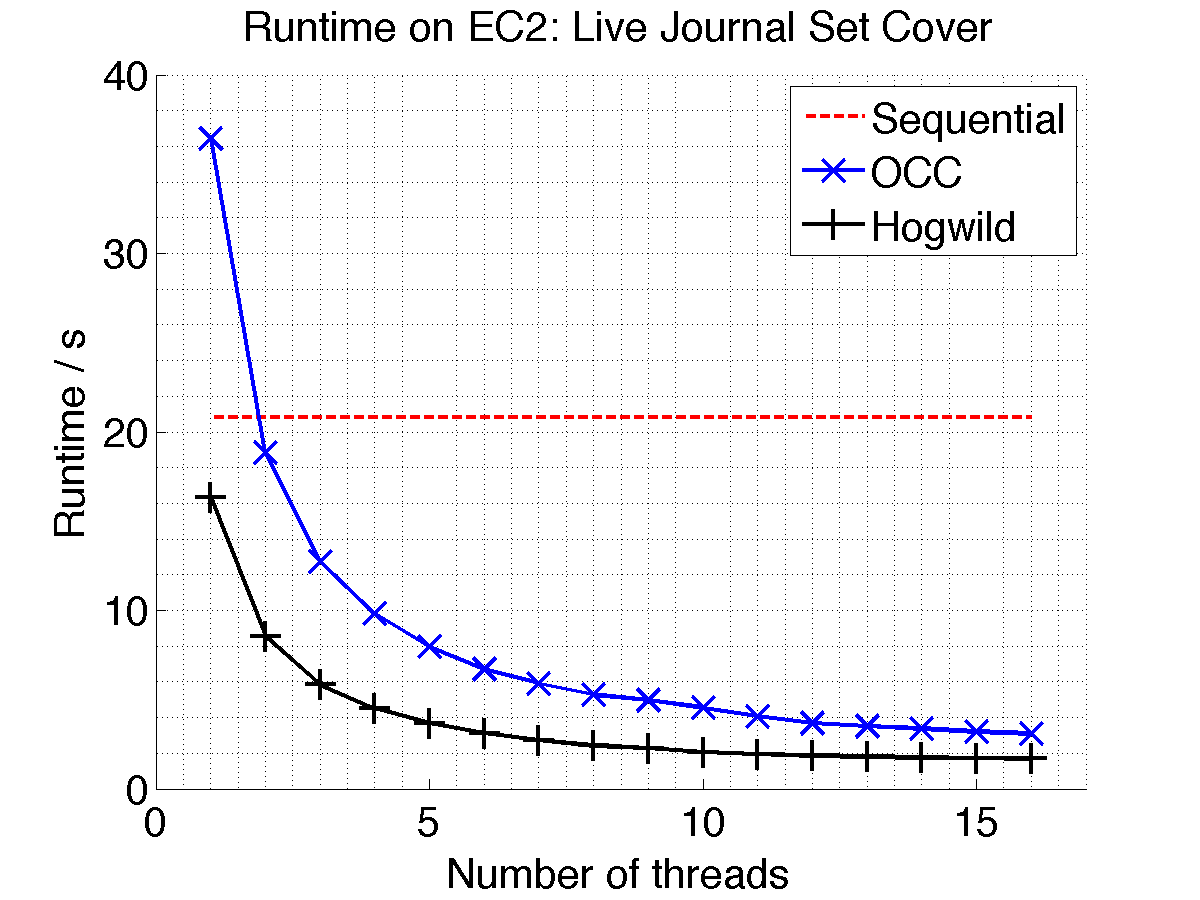
\includegraphics[width=150pt]{images/runtime_livejournal_setcover.png}
			\caption{Runtime, Live Journal}
			\label{fig:runtime_livejournal_setcover}
	  \end{subfigure} \\
	  \begin{subfigure}[b]{0.31\textwidth}
	  	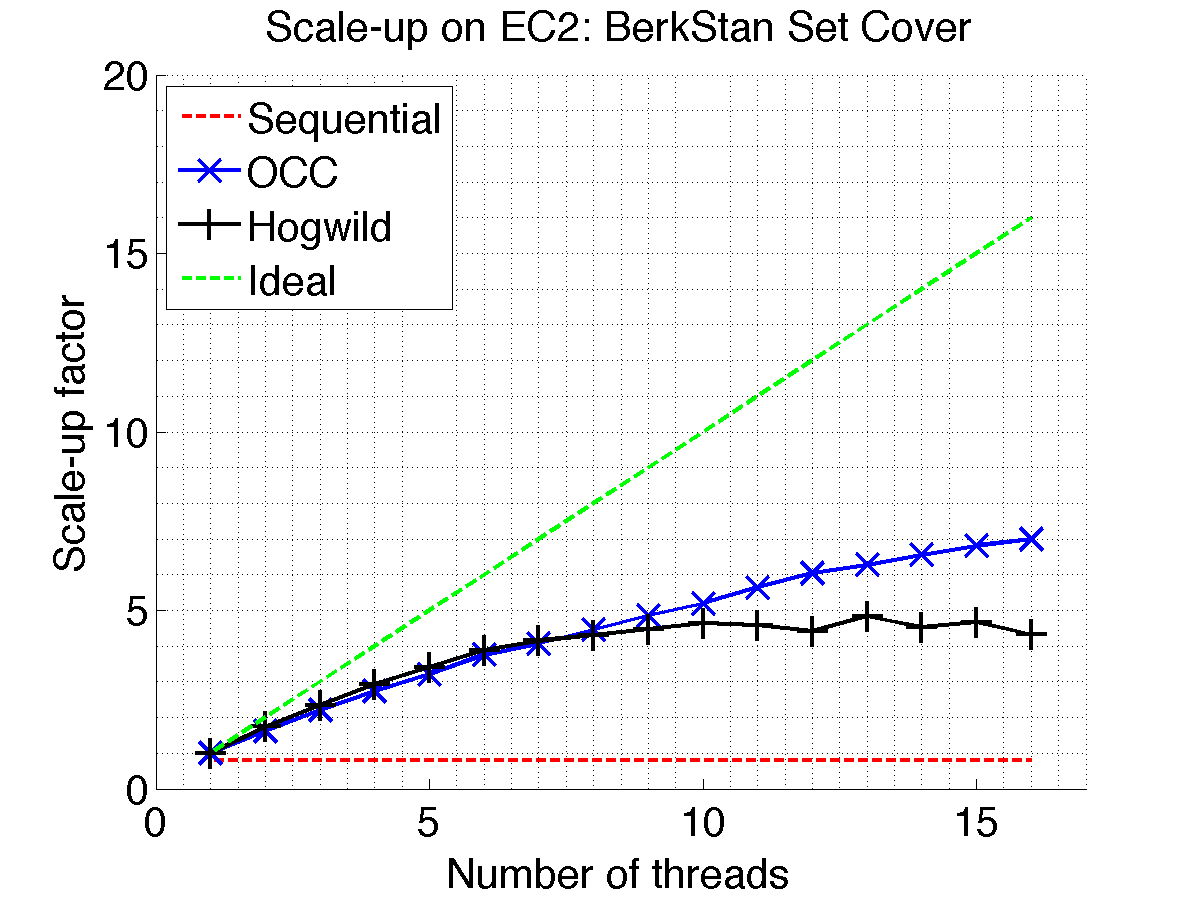
\includegraphics[width=150pt]{images/scaleup_webberkstan_setcover.png}
			\caption{Scale-up, BerkStan}
			\label{fig:scaleup_webberkstan_setcover}
	  \end{subfigure} &
	  \begin{subfigure}[b]{0.31\textwidth}
	  	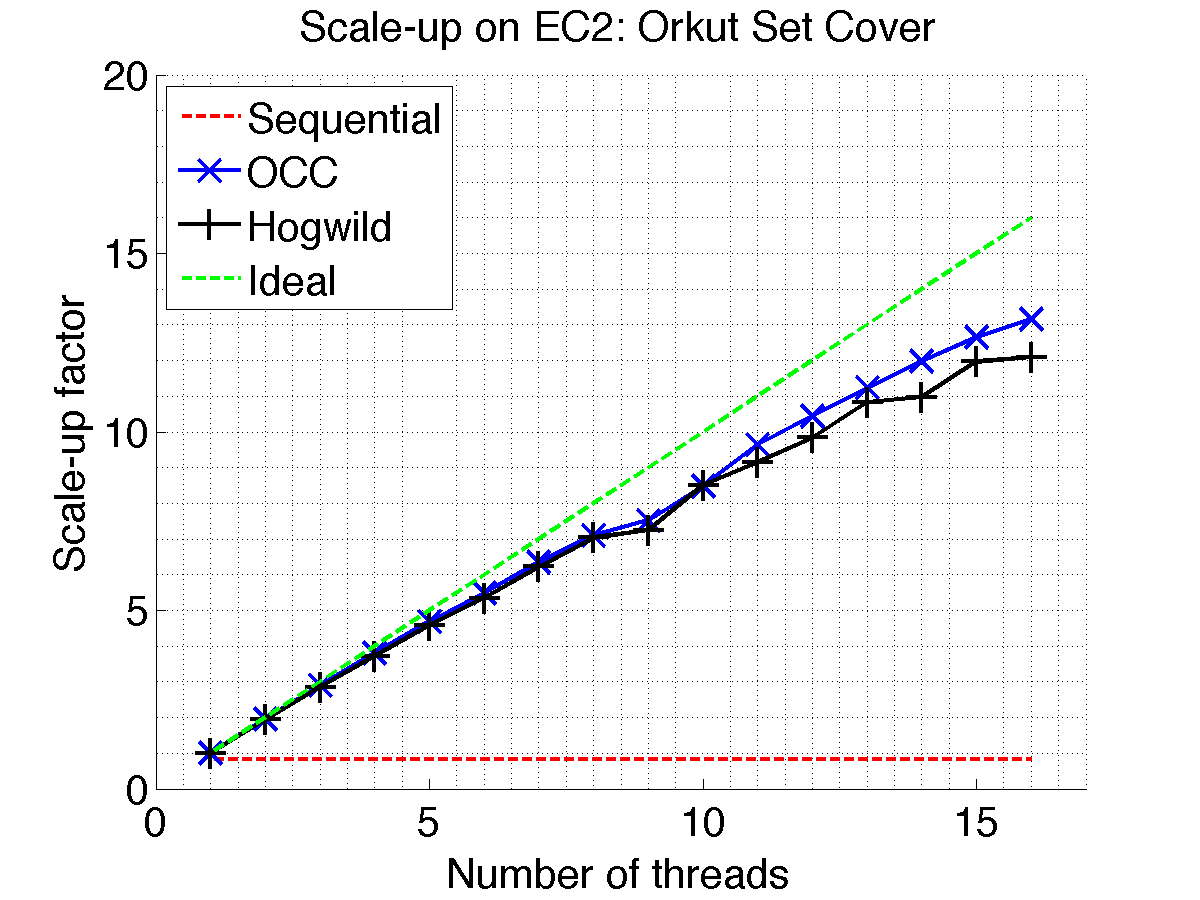
\includegraphics[width=150pt]{images/scaleup_orkut_setcover.png}
			\caption{Scale-up, Orkut}
			\label{fig:scaleup_orkut_setcover}
	  \end{subfigure} &
	  \begin{subfigure}[b]{0.31\textwidth}
	  	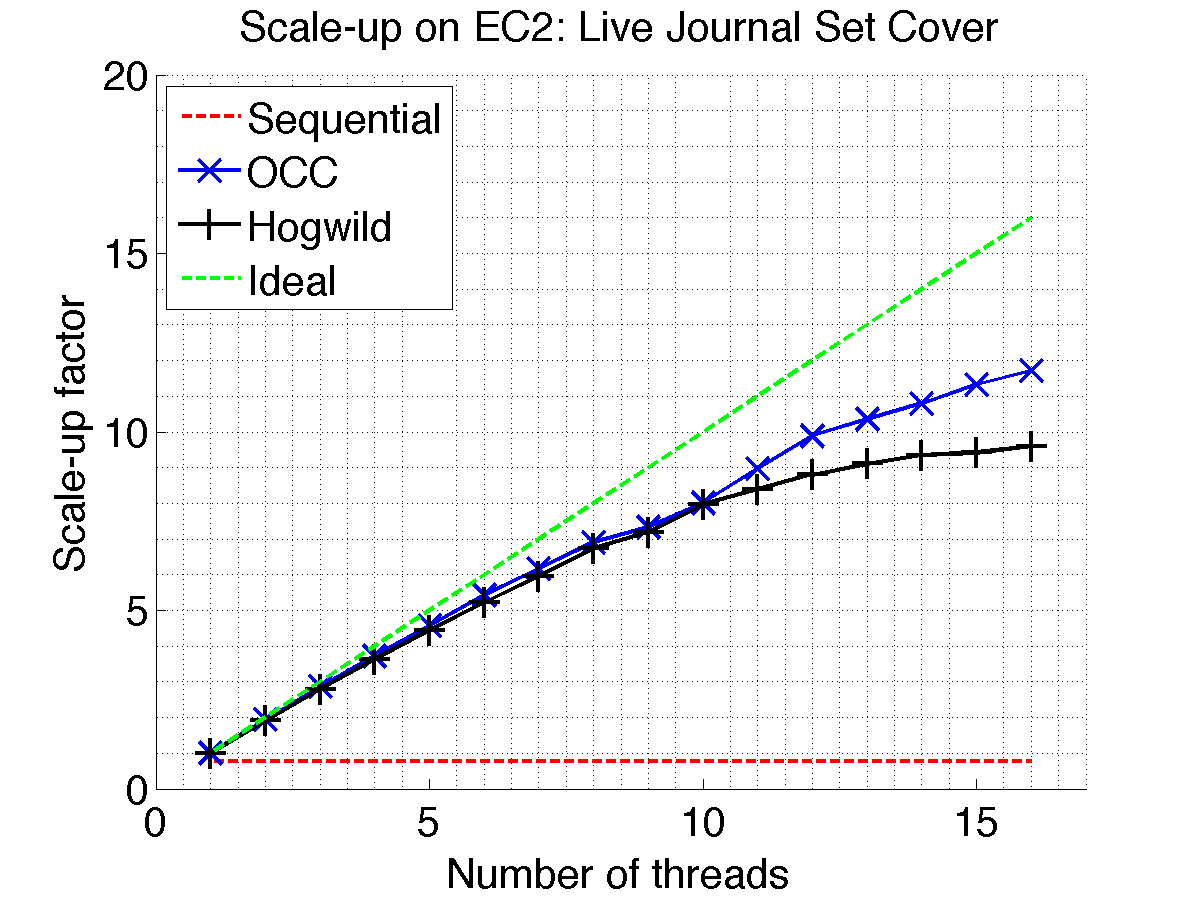
\includegraphics[width=150pt]{images/scaleup_livejournal_setcover.png}
			\caption{Scale-up, Live Journal}
			\label{fig:scaleup_livejournal_setcover}
	  \end{subfigure} \\
	  \begin{subfigure}[b]{0.31\textwidth}
	  	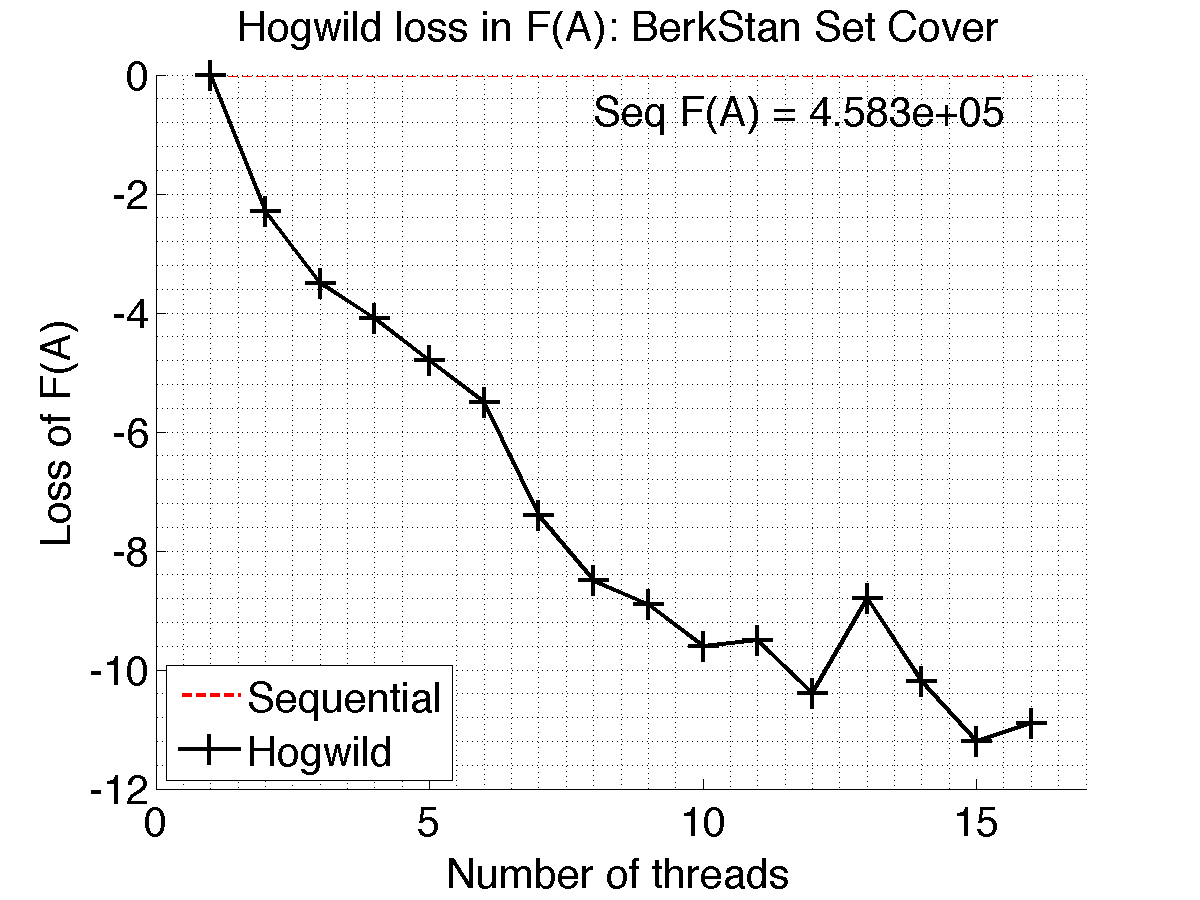
\includegraphics[width=150pt]{images/diffFA_Hogwild_webberkstan_setcover.png}
			\caption{Hogwild $F(A)$, BerkStan}
			\label{fig:diffFA_Hogwild_webberkstan_setcover}
	  \end{subfigure} &
	  \begin{subfigure}[b]{0.31\textwidth}
	  	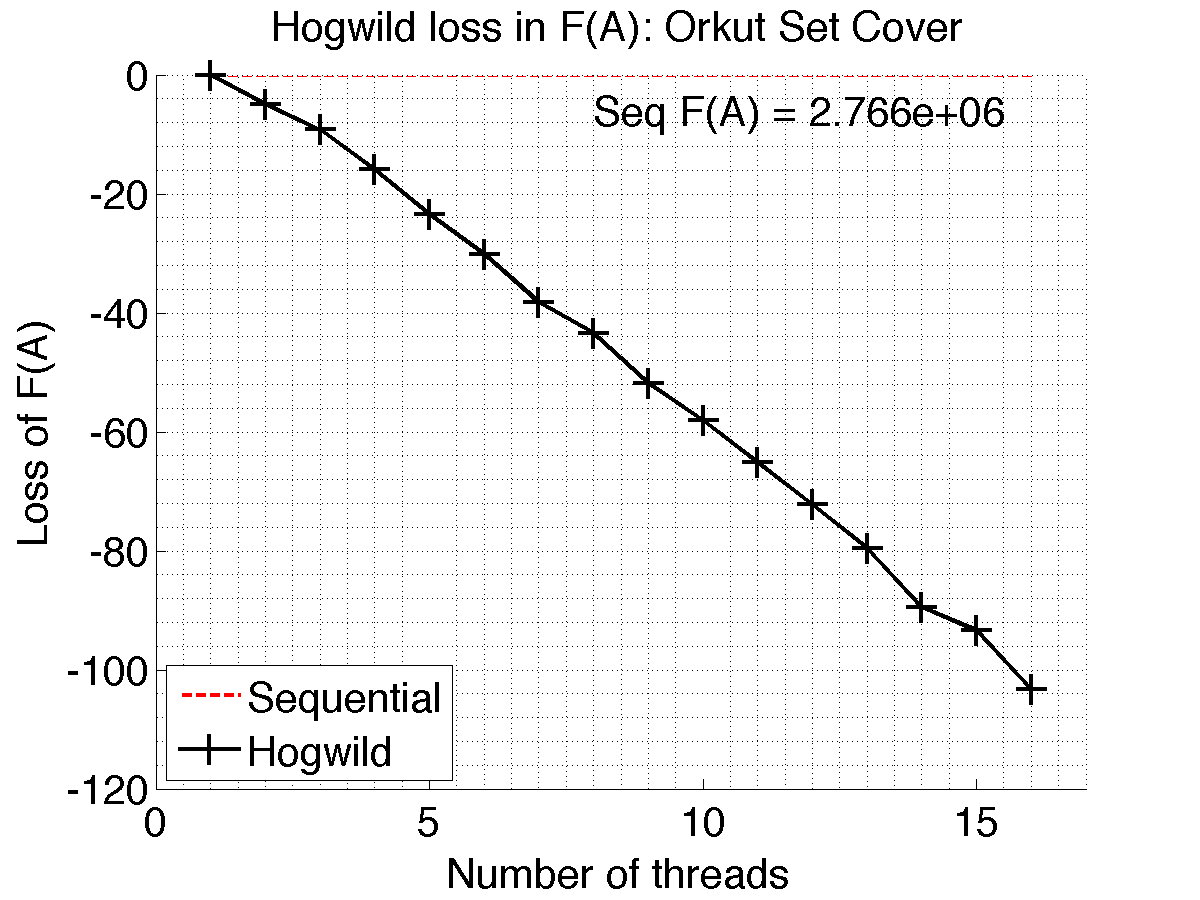
\includegraphics[width=150pt]{images/diffFA_Hogwild_orkut_setcover.png}
			\caption{Hogwild $F(A)$, Orkut}
			\label{fig:diffFA_Hogwild_orkut_setcover}
	  \end{subfigure} &
	  \begin{subfigure}[b]{0.31\textwidth}
	  	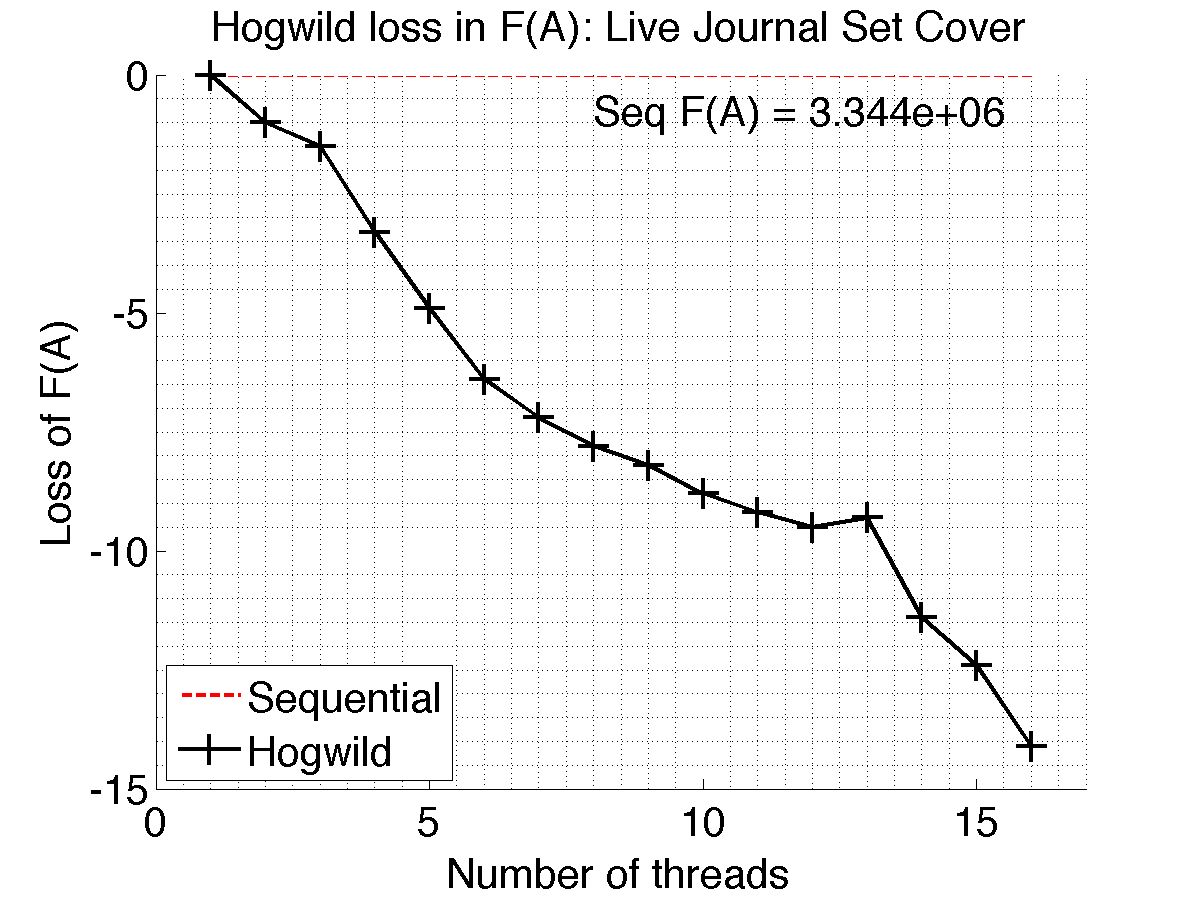
\includegraphics[width=150pt]{images/diffFA_Hogwild_livejournal_setcover.png}
			\caption{Hogwild $F(A)$, Live Journal}
			\label{fig:diffFA_Hogwild_livejournal_setcover}
	  \end{subfigure} \\
	  \begin{subfigure}[b]{0.31\textwidth}
	  	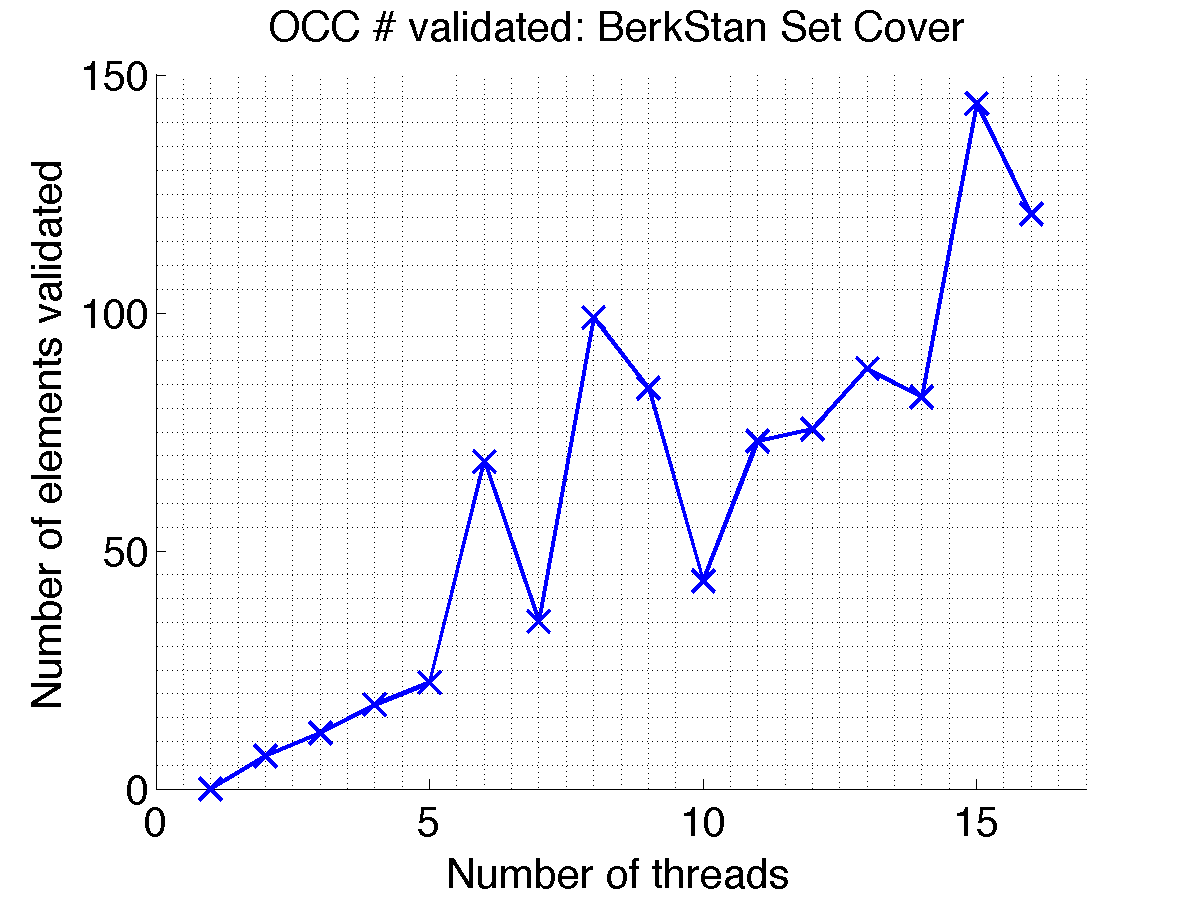
\includegraphics[width=150pt]{images/validated_OCC_webberkstan_setcover.png}
			\caption{OCC \# validated, BerkStan}
			\label{fig:validated_OCC_webberkstan_setcover}
	  \end{subfigure} &
	  \begin{subfigure}[b]{0.31\textwidth}
	  	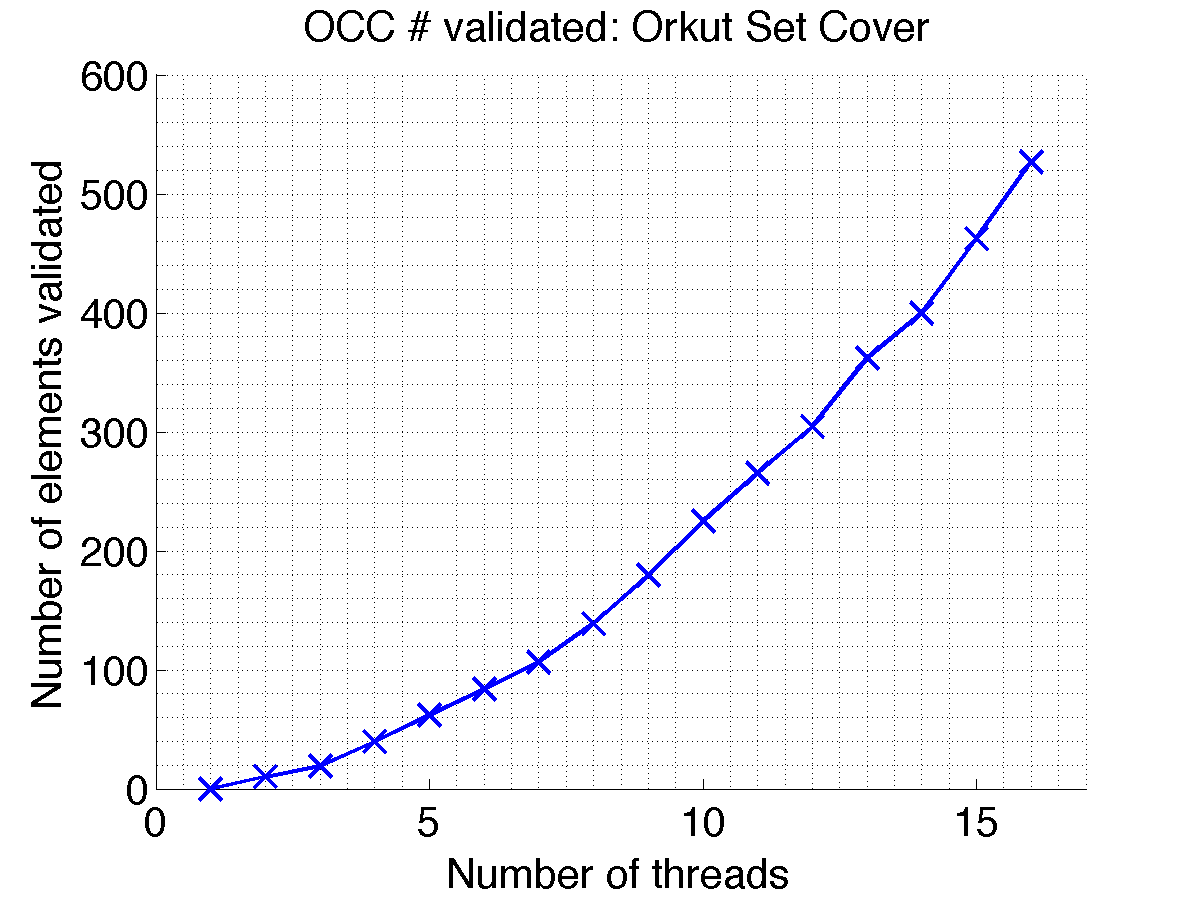
\includegraphics[width=150pt]{images/validated_OCC_orkut_setcover.png}
			\caption{OCC \# validated, Orkut}
			\label{fig:validated_OCC_orkut_setcover}
	  \end{subfigure} &
	  \begin{subfigure}[b]{0.31\textwidth}
	  	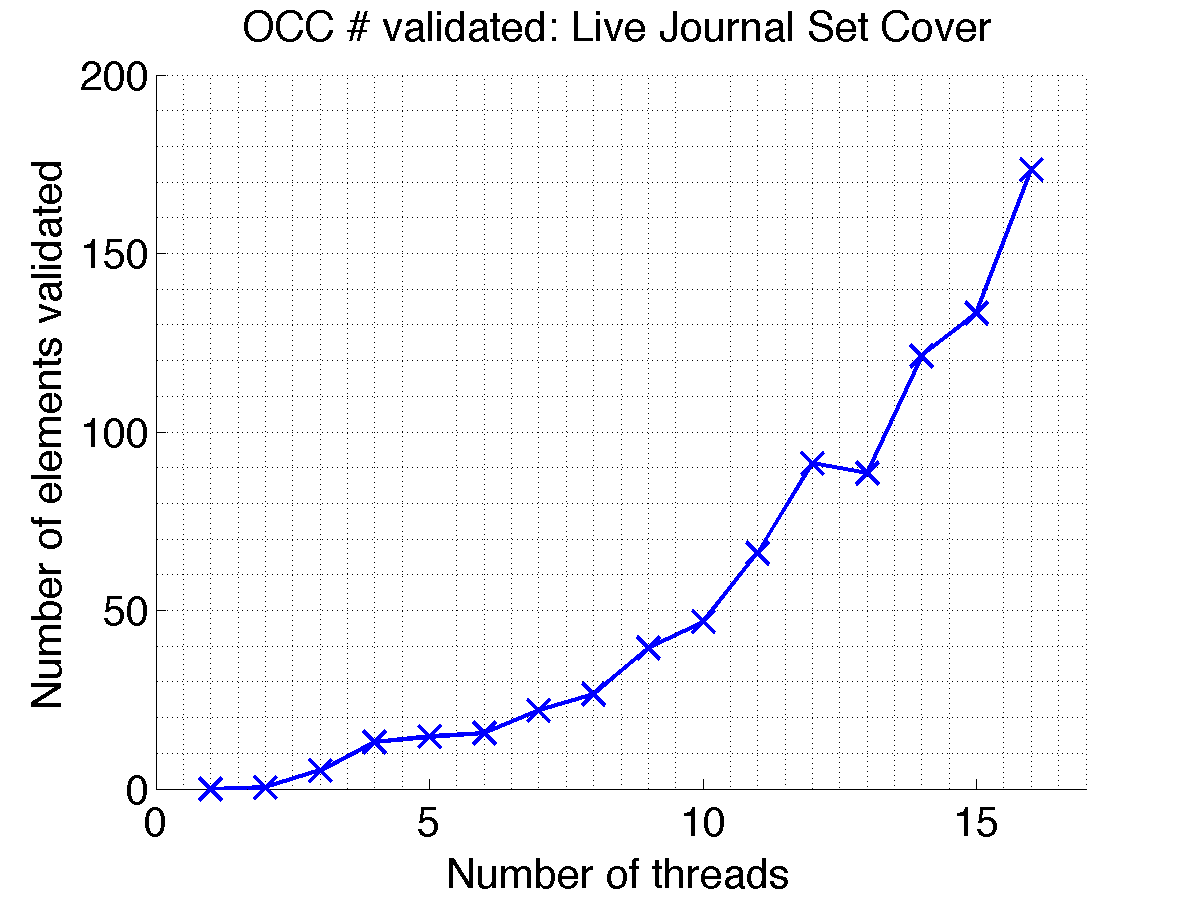
\includegraphics[width=150pt]{images/validated_OCC_livejournal_setcover.png}
			\caption{OCC \# validated, Live Journal}
			\label{fig:validated_OCC_livejournal_setcover}
	  \end{subfigure} \\
  \end{tabular}
  \caption{Set cover on 3 real graphs.}
\end{figure}



\begin{figure}[ht]
  \centering
  \begin{tabular}{ccc}
	  \begin{subfigure}[b]{0.31\textwidth}
	  	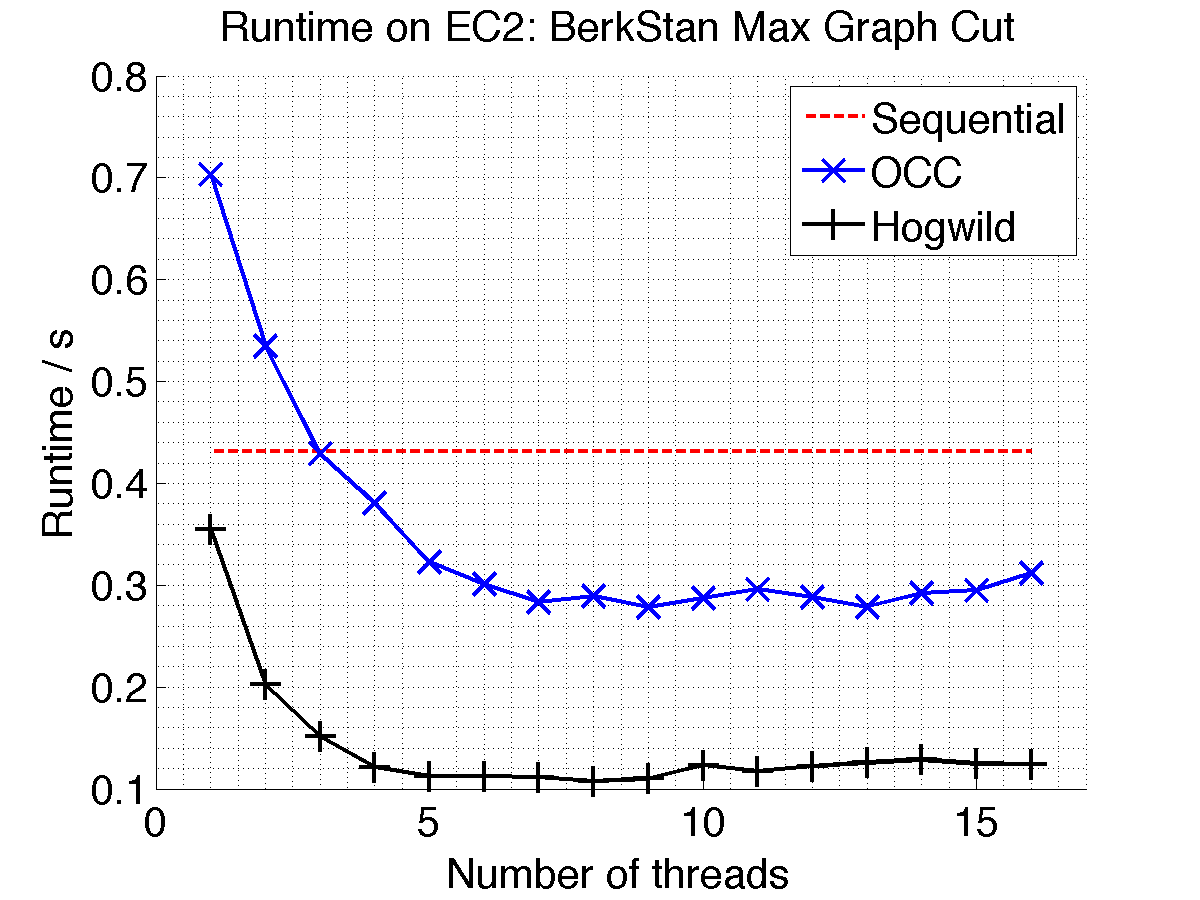
\includegraphics[width=150pt]{images/runtime_webberkstan_maxgraphcut.png}
			\caption{Runtime, BerkStan}
			\label{fig:runtime_webberkstan_maxgraphcut}
	  \end{subfigure} &
	  \begin{subfigure}[b]{0.31\textwidth}
	  	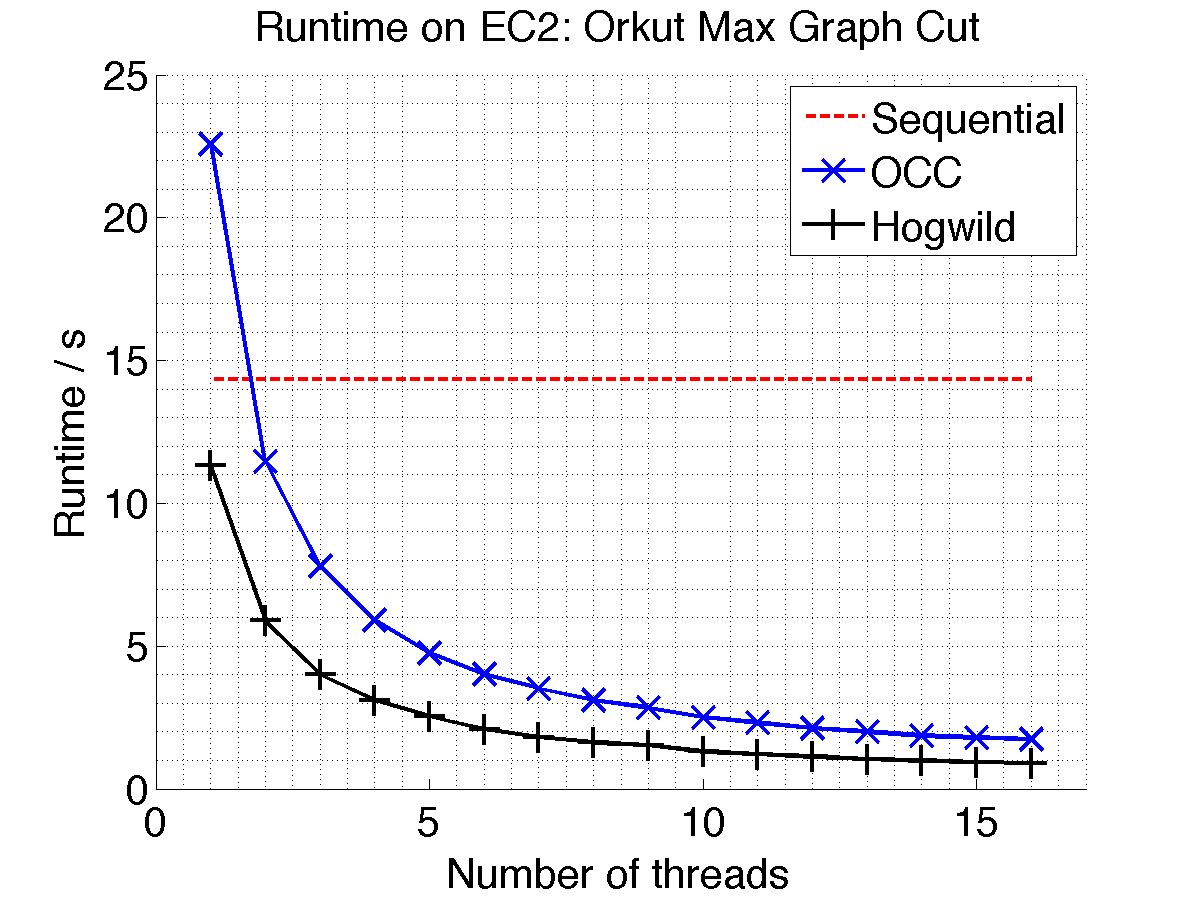
\includegraphics[width=150pt]{images/runtime_orkut_maxgraphcut.png}
			\caption{Runtime, Orkut}
			\label{fig:runtime_orkut_maxgraphcut}
	  \end{subfigure} &
	  \begin{subfigure}[b]{0.31\textwidth}
	  	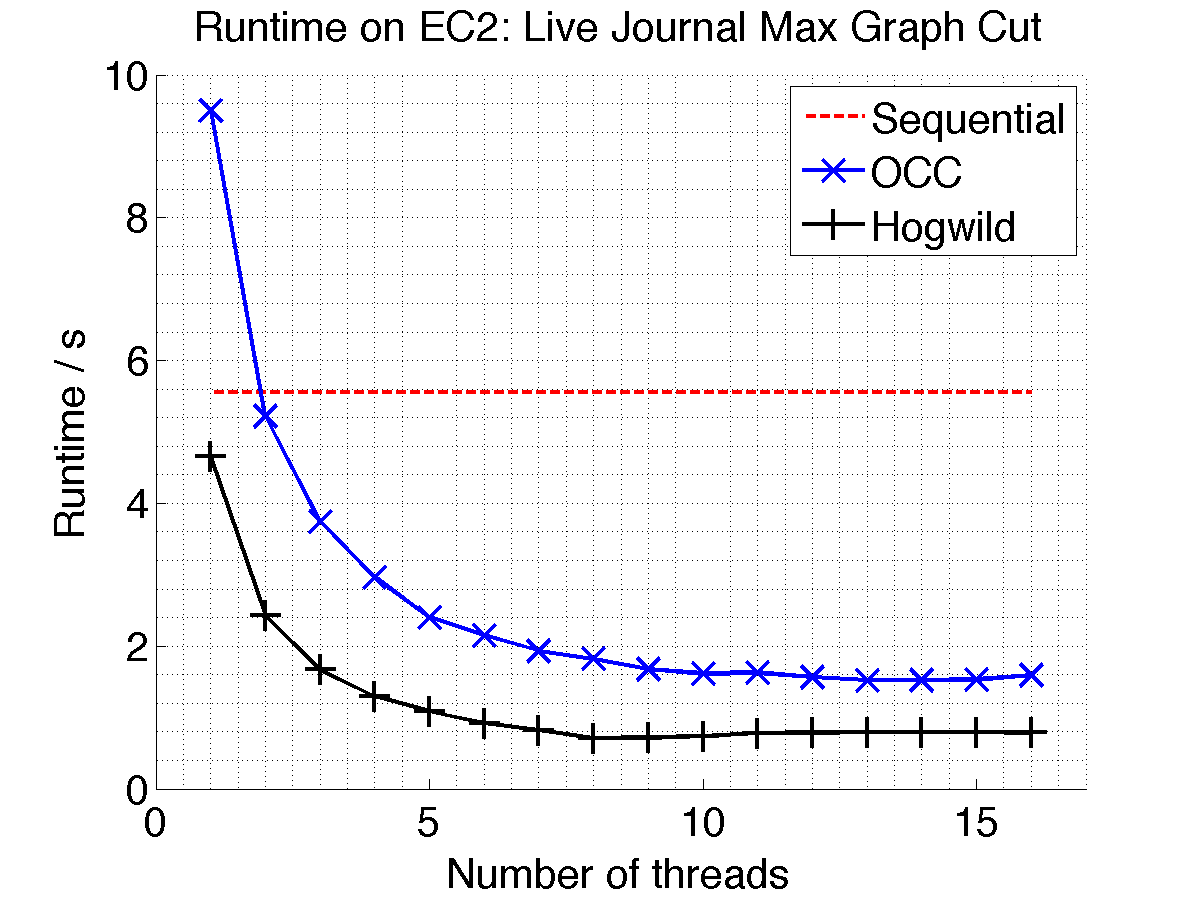
\includegraphics[width=150pt]{images/runtime_livejournal_maxgraphcut.png}
			\caption{Runtime, Live Journal}
			\label{fig:runtime_livejournal_maxgraphcut}
	  \end{subfigure} \\
	  \begin{subfigure}[b]{0.31\textwidth}
	  	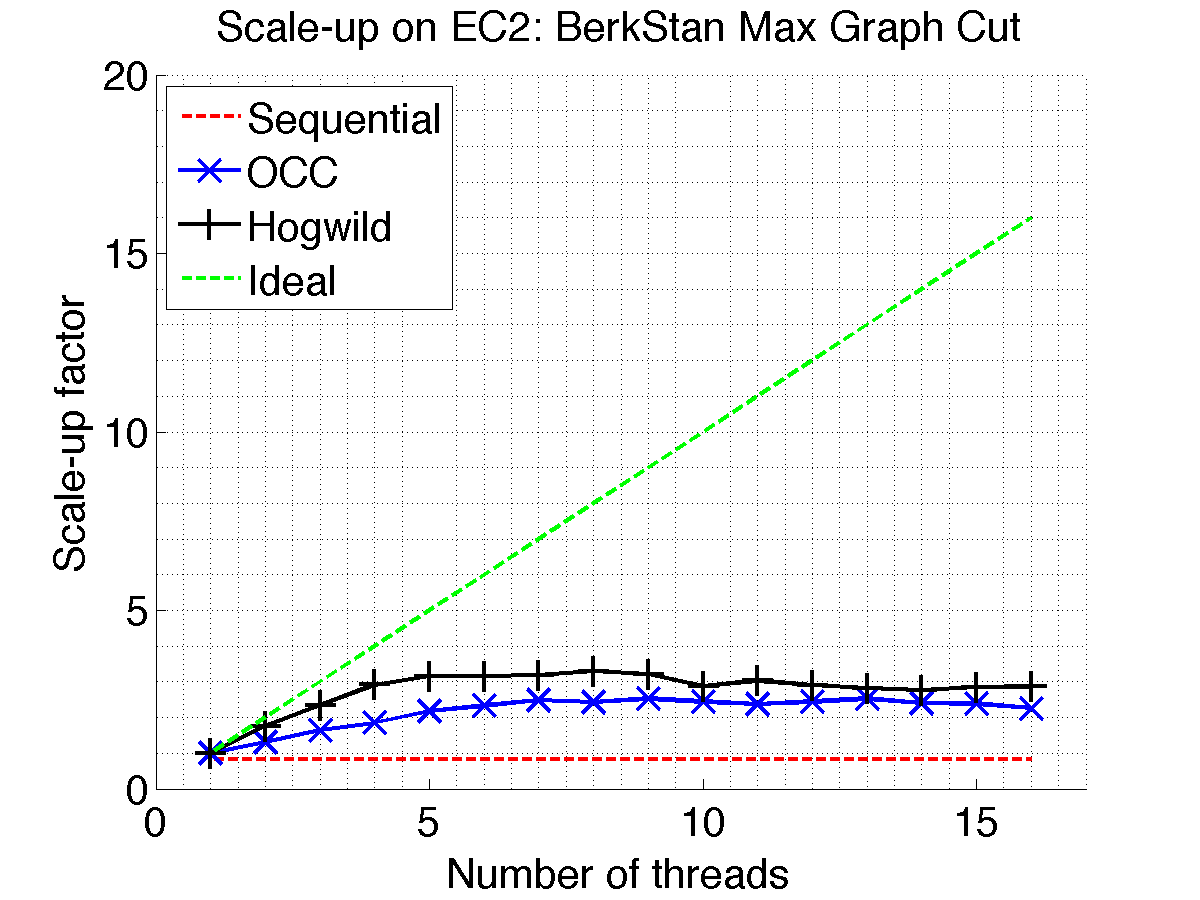
\includegraphics[width=150pt]{images/scaleup_webberkstan_maxgraphcut.png}
			\caption{Scale-up, BerkStan}
			\label{fig:scaleup_webberkstan_maxgraphcut}
	  \end{subfigure} &
	  \begin{subfigure}[b]{0.31\textwidth}
	  	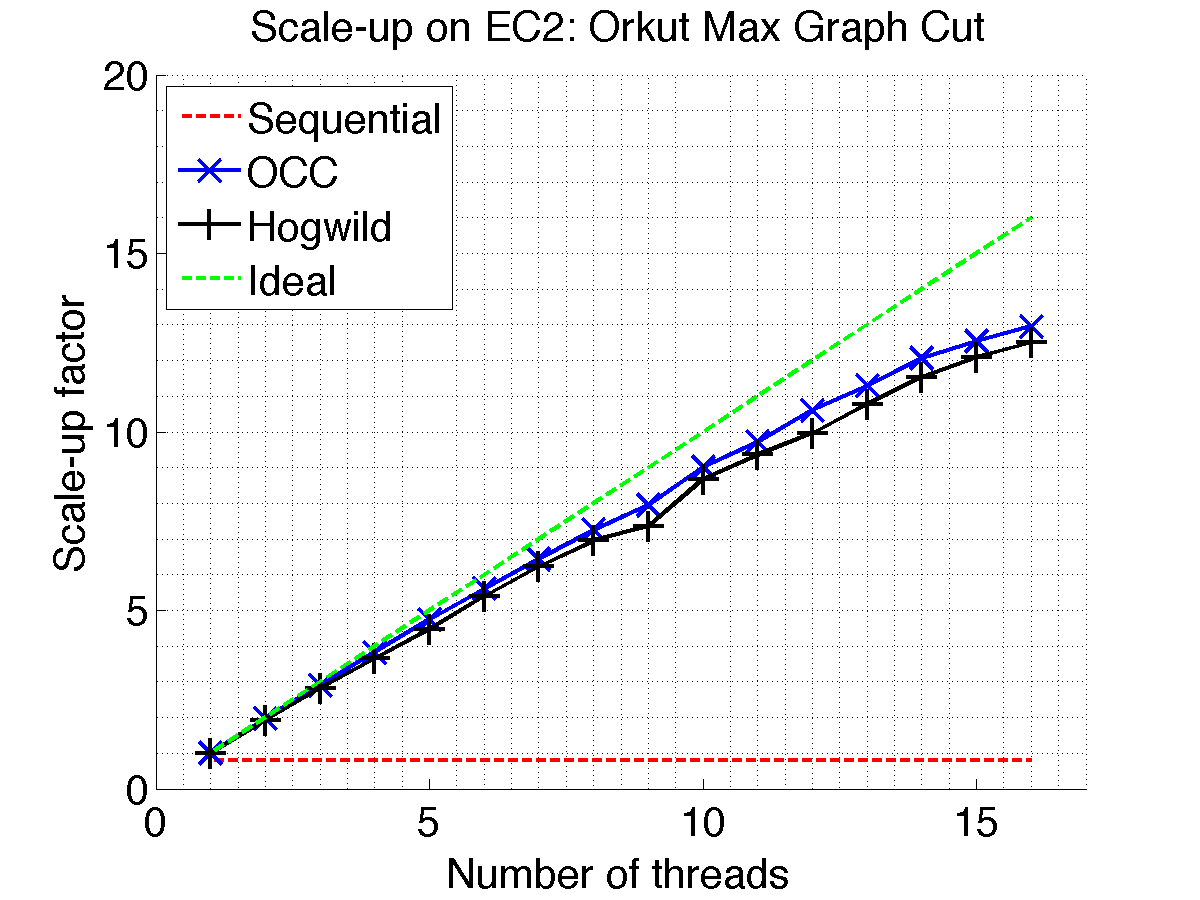
\includegraphics[width=150pt]{images/scaleup_orkut_maxgraphcut.png}
			\caption{Scale-up, Orkut}
			\label{fig:scaleup_orkut_maxgraphcut}
	  \end{subfigure} &
	  \begin{subfigure}[b]{0.31\textwidth}
	  	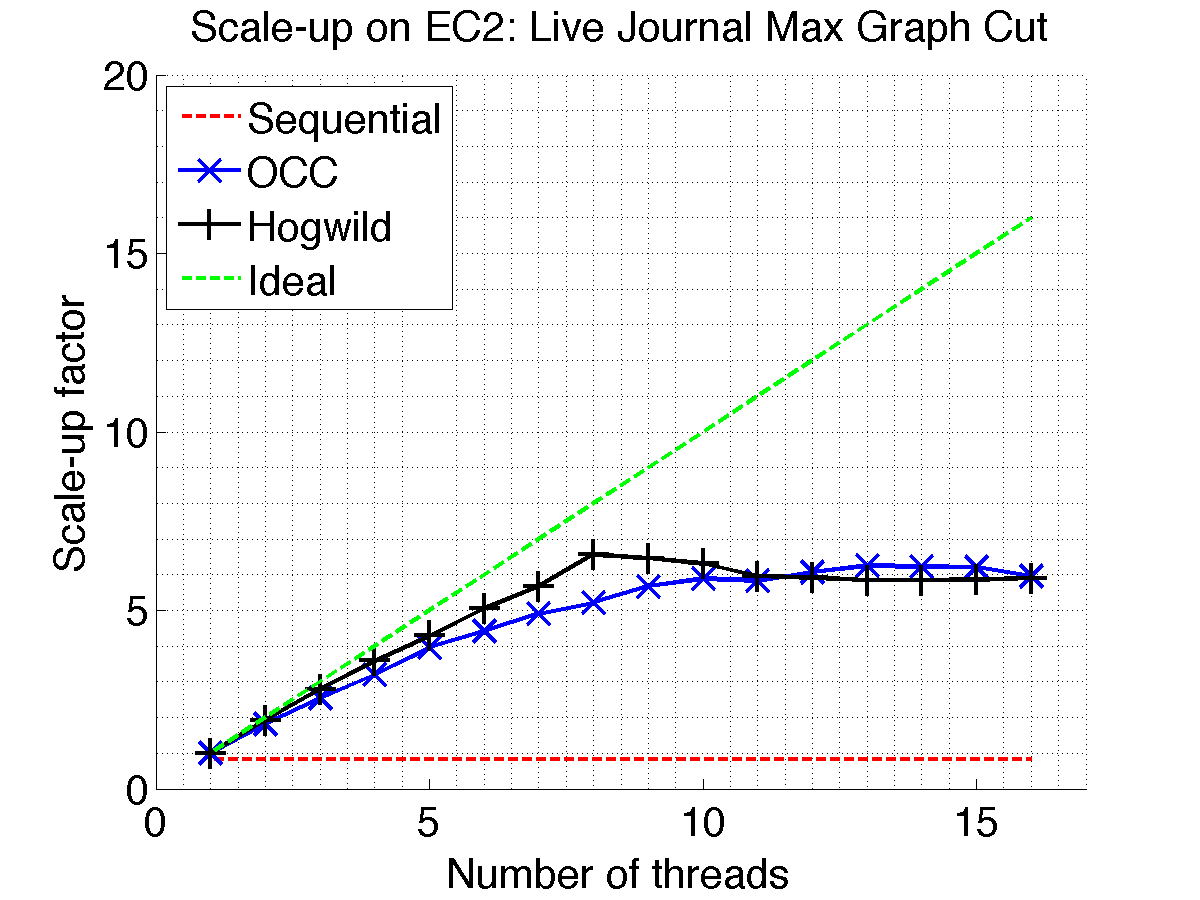
\includegraphics[width=150pt]{images/scaleup_livejournal_maxgraphcut.png}
			\caption{Scale-up, Live Journal}
			\label{fig:scaleup_livejournal_maxgraphcut}
	  \end{subfigure} \\
	  \begin{subfigure}[b]{0.31\textwidth}
	  	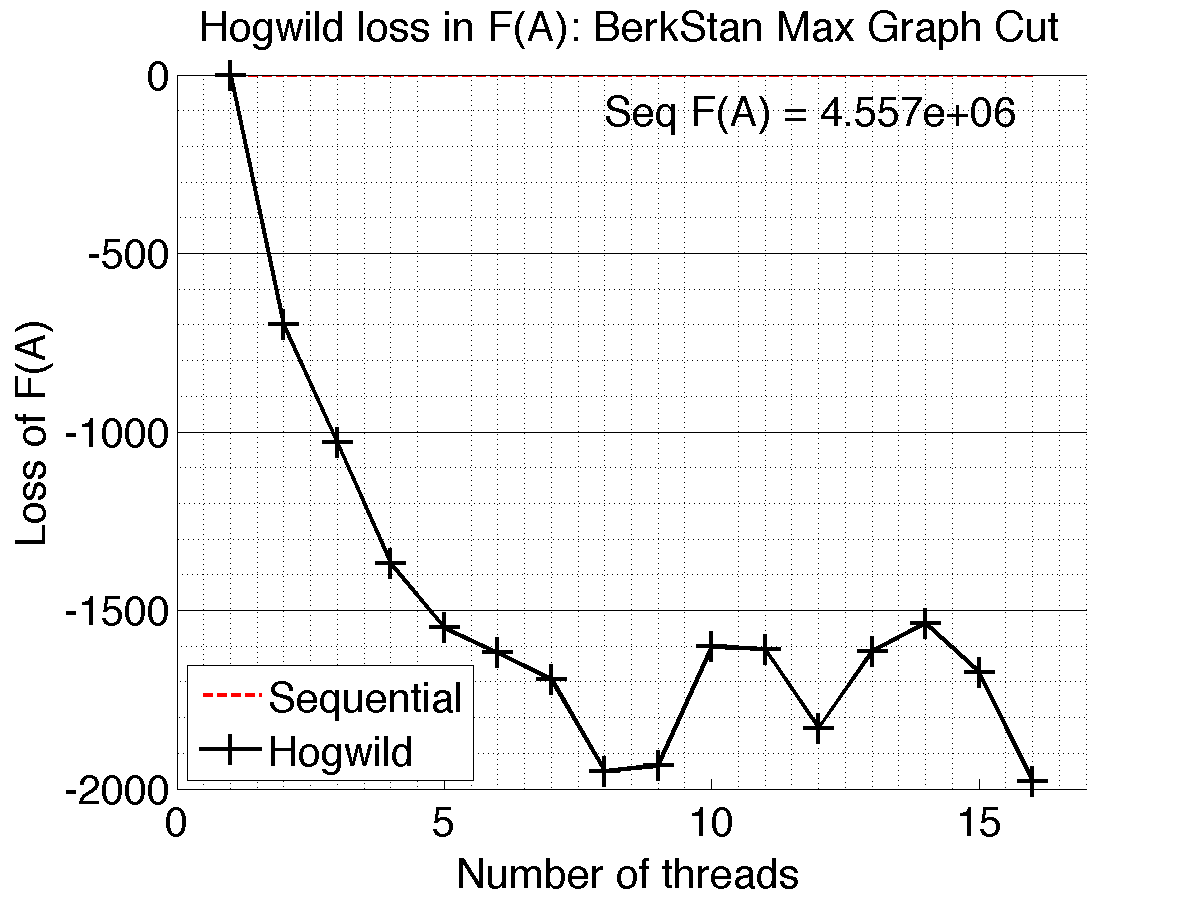
\includegraphics[width=150pt]{images/diffFA_Hogwild_webberkstan_maxgraphcut.png}
			\caption{Hogwild $F(A)$, BerkStan}
			\label{fig:diffFA_Hogwild_webberkstan_maxgraphcut}
	  \end{subfigure} &
	  \begin{subfigure}[b]{0.31\textwidth}
	  	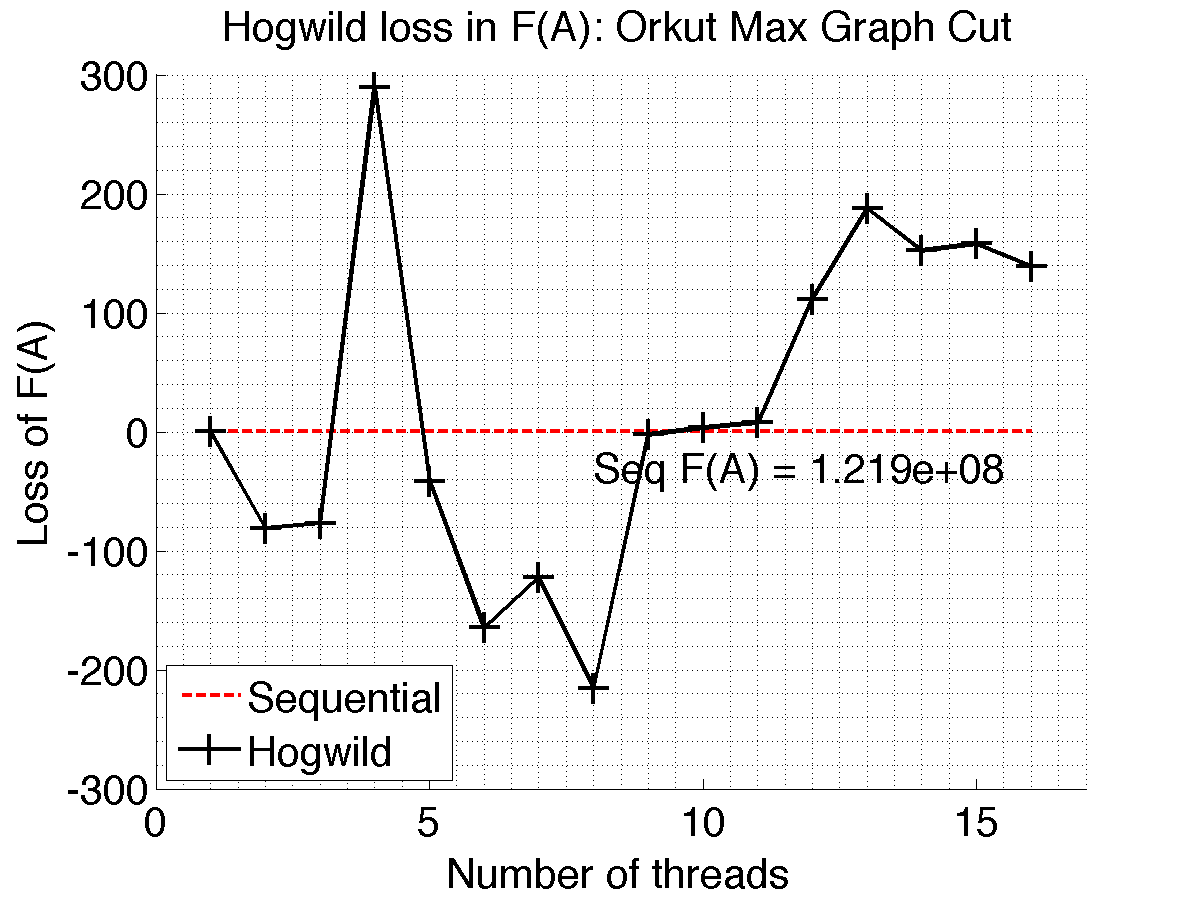
\includegraphics[width=150pt]{images/diffFA_Hogwild_orkut_maxgraphcut.png}
			\caption{Hogwild $F(A)$, Orkut}
			\label{fig:diffFA_Hogwild_orkut_maxgraphcut}
	  \end{subfigure} &
	  \begin{subfigure}[b]{0.31\textwidth}
	  	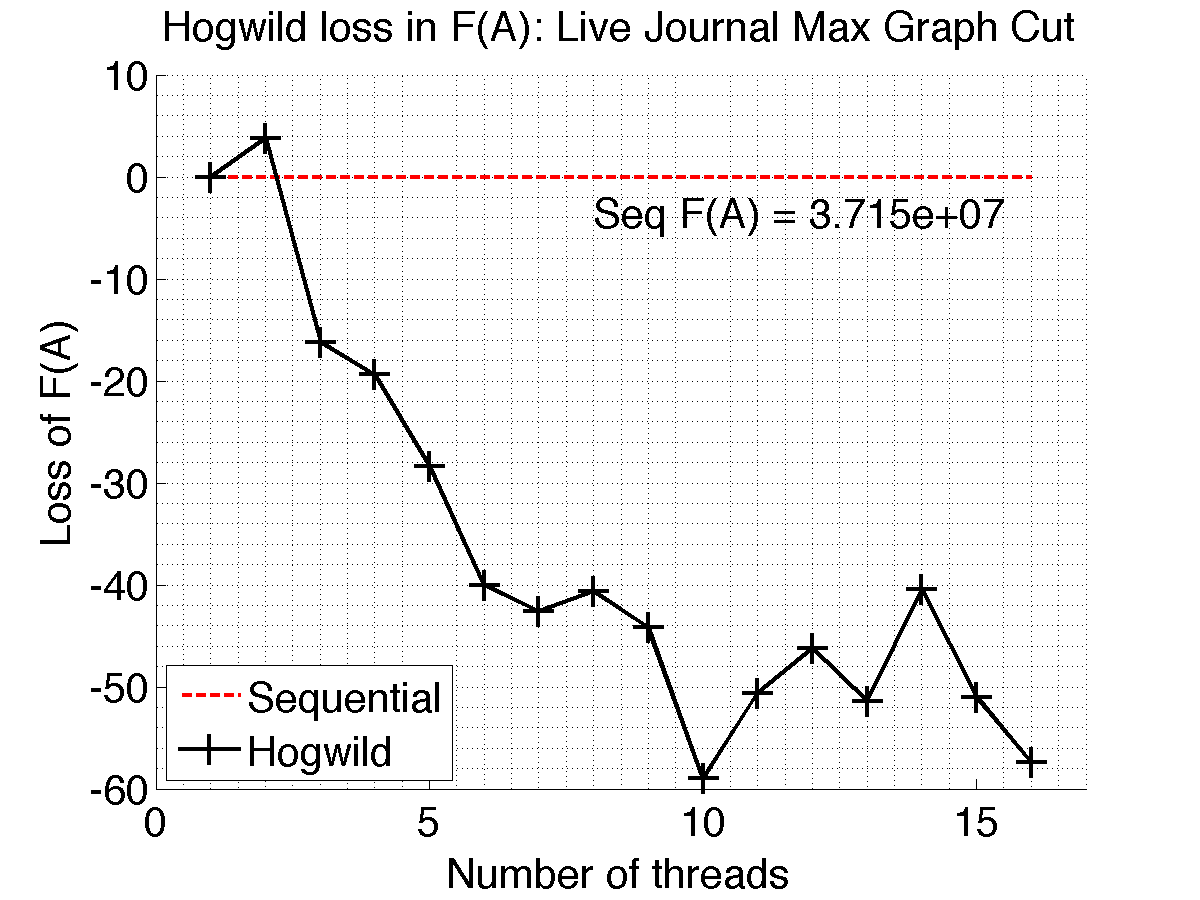
\includegraphics[width=150pt]{images/diffFA_Hogwild_livejournal_maxgraphcut.png}
			\caption{Hogwild $F(A)$, Live Journal}
			\label{fig:diffFA_Hogwild_livejournal_maxgraphcut}
	  \end{subfigure} \\
	  \begin{subfigure}[b]{0.31\textwidth}
	  	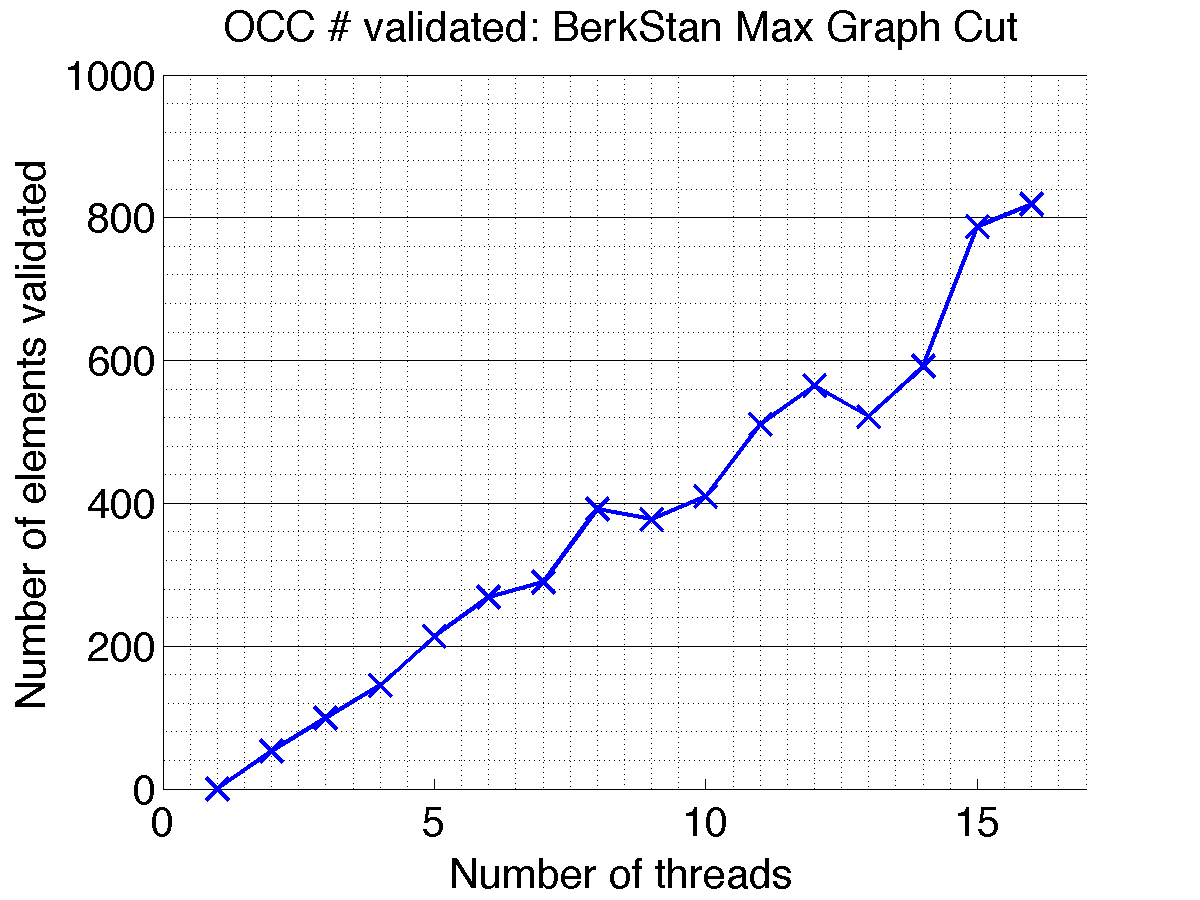
\includegraphics[width=150pt]{images/validated_OCC_webberkstan_maxgraphcut.png}
			\caption{OCC \# validated, BerkStan}
			\label{fig:validated_OCC_webberkstan_maxgraphcut}
	  \end{subfigure} &
	  \begin{subfigure}[b]{0.31\textwidth}
	  	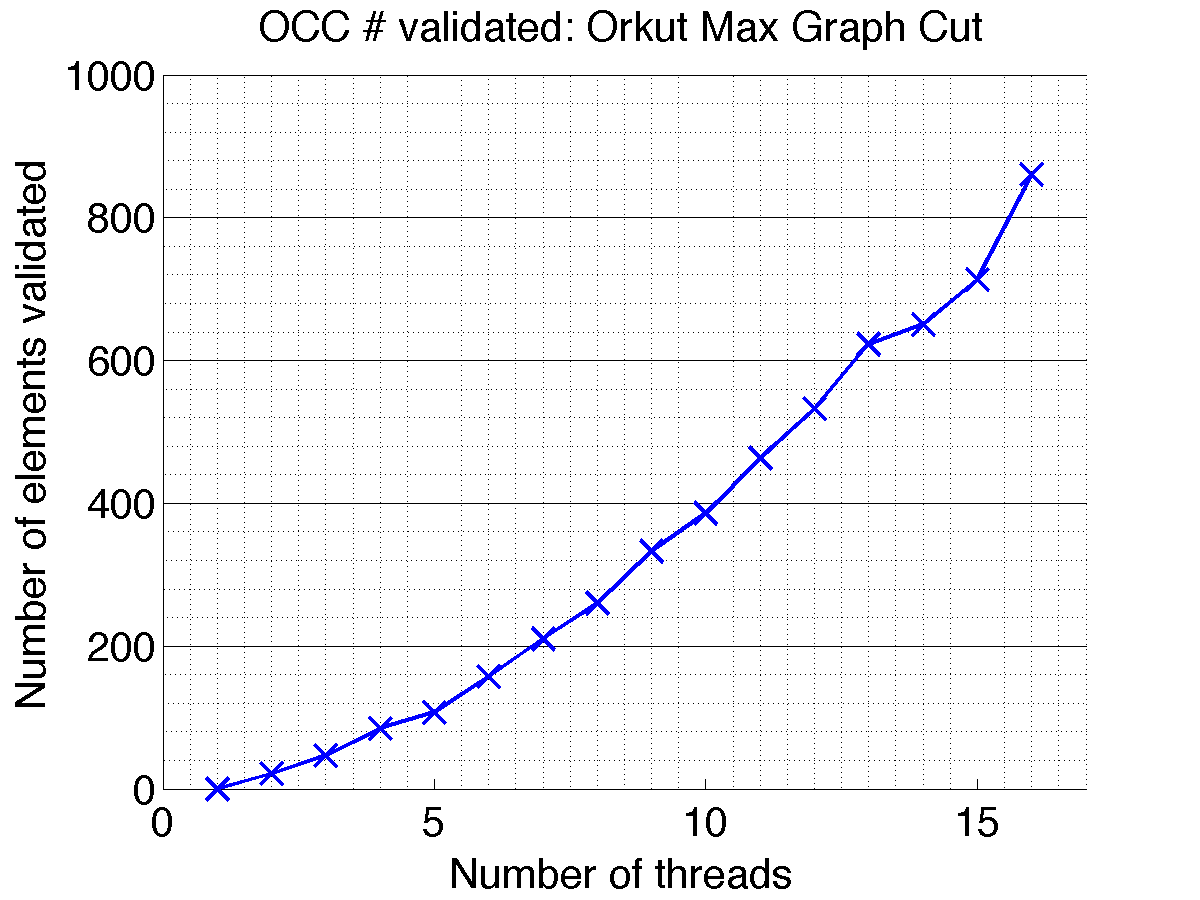
\includegraphics[width=150pt]{images/validated_OCC_orkut_maxgraphcut.png}
			\caption{OCC \# validated, Orkut}
			\label{fig:validated_OCC_orkut_maxgraphcut}
	  \end{subfigure} &
	  \begin{subfigure}[b]{0.31\textwidth}
	  	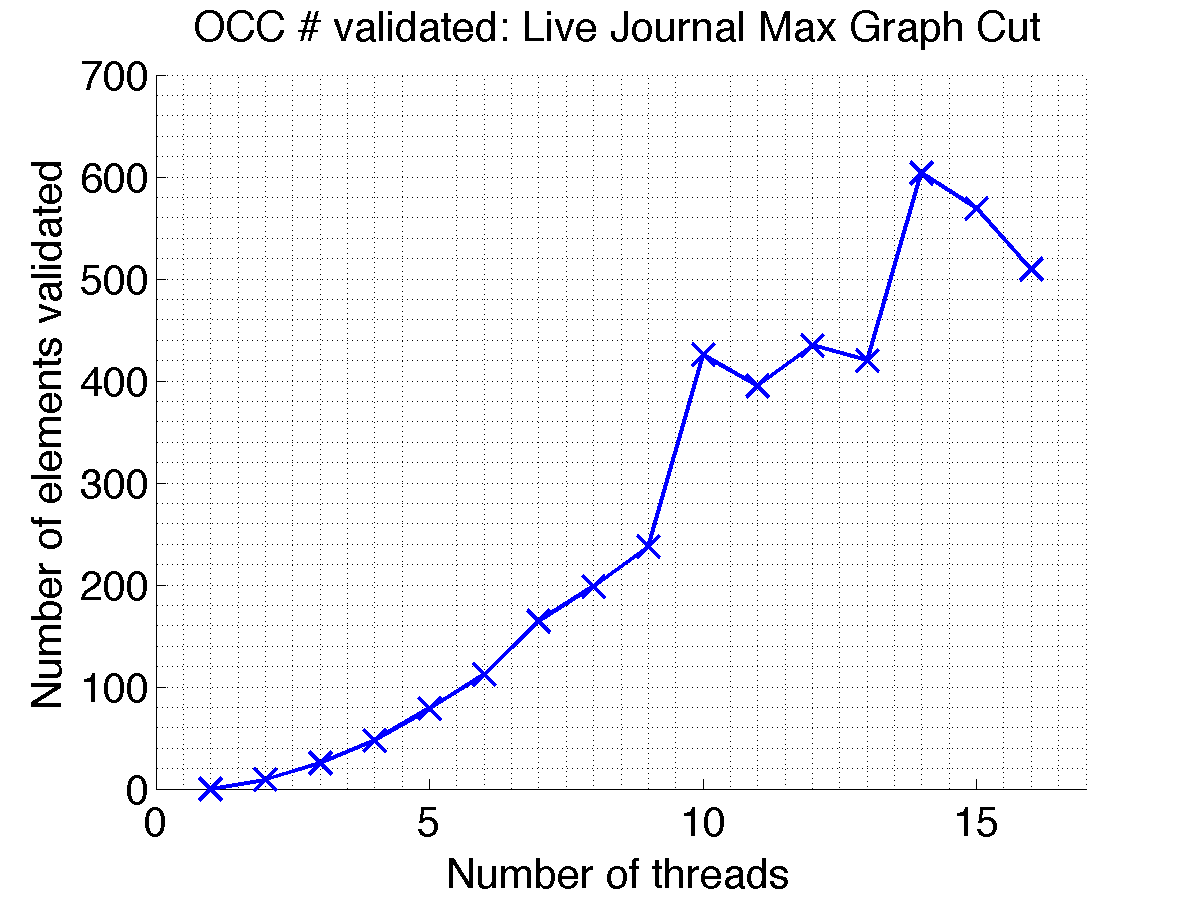
\includegraphics[width=150pt]{images/validated_OCC_livejournal_maxgraphcut.png}
			\caption{OCC \# validated, Live Journal}
			\label{fig:validated_OCC_livejournal_maxgraphcut}
	  \end{subfigure} \\
  \end{tabular}
  \caption{Max graph cut on 3 real graphs.}
\end{figure}



\section{Discussions}

{\footnotesize
%\subsection*{Acknowledgments}
%This research is supported in part by NSF CISE Expeditions award CCF-1139158 and DARPA XData Award FA8750-12-2-0331, and  gifts from Amazon Web Services, Google, SAP,  Blue Goji, Cisco, Clearstory Data, Cloudera, Ericsson, Facebook, General Electric, Hortonworks, Intel, Microsoft, NetApp, Oracle, Samsung, Splunk, VMware and Yahoo!.
%This material is also based upon work supported in part by the Office of
%Naval Research under contract/grant number N00014-11-1-0688. 
%X. Pan's work is also supported in part by a DSO National Laboratories Postgraduate Scholarship.

% In the unusual situation where you want a paper to appear in the
% references without citing it in the main text, use \nocite
%\nocite{langley00}

\bibliographystyle{unsrtnat}
\bibliography{references_arxiv}
}

\newpage
\appendix

\section{Proof of bound for \hogwild{}}
\label{app:proofhogwild}


We follow the proof outline of \cite{buchbinder2012}.

Consider an ordering $\iota$ inducted by running \hogwild{}.
For convenience, we will use $i$ to flexibly denote the element $e$ and its ordering $\iota(e)$.

Let $OPT$ be an optimal solution to the problem.
Define $O^i := (OPT \cup A^i) \cap B^i$.
Note that $O^i$ coincides with $A^i$ and $B^i$ on elements $1,\dots,i$, and $O^i$ coincides with $OPT$ on elements $i+1,\dots, n$.
Hence,
\begin{align*}
O^i \backslash i+1 &\supseteq A^i \text{\stef{Is this $(i+1)$ or adding one?}}\\
O^i \cup i+1 &\subseteq B^i.
\end{align*}

\begin{lem}\label{lem:positivesum} For every $1 \leq i \leq n$, $\Delta_+(i) + \Delta_-(i) \geq 0$.
\end{lem}
\begin{proof} This is just Lemma II.1 of \cite{buchbinder2012}.
\end{proof}

\begin{lem}\label{lem:singleelement}
Let $\rho_i = \max\{\Delta_+^{\max}(e) - \Delta_+(e), \Delta_-^{\max}(e) - \Delta_-(e)\}$.
For every $1 \leq i \leq n$,
\[E[F(O^{i-1})-F(O^i)] \leq \frac{1}{2} E[F(A^i) - F(A^{i-1}) + F(B^i) - F(B^{i-1}) + \rho_i].\]
\end{lem}
\begin{proof}
We follow the proof outline of \cite{buchbinder2012}.
First, note that it suffices to prove the inequality conditioned on knowing $A^{i-1}$, $\hat{A}_i$ and $\hat{B}_i$, then applying the law of total expectation.
Under this conditioning, we also know $B^{i-1}$, $O^{i-1}$, $\Delta_+(i)$, $\Delta_+^{\max}(i)$, $\Delta_-(i)$, and $\Delta_-^{\max}(i)$.



We consider the following 6 cases.


\begin{description}

\item\textbf{Case 1:} $0 < \Delta_+(i) \leq \Delta_+^{\max}(i)$, $0 \leq \Delta_-^{\max}(i)$.
Since both $\Delta_+^{\max}(i)>0$ and $\Delta_-^{\max}(i)>0$, the probability of including $i$ is just $\Delta_+^{\max}(i) / (\Delta_+^{\max}(i) + \Delta_-^{\max}(i))$, and the probability of excluding $i$ is $\Delta_-^{\max}(i) / (\Delta_+^{\max}(i) + \Delta_-^{\max}(i))$.
\begin{align*}
E[F(A^i) - F(A^{i-1}) | A^{i-1}, \hat{A}_i, \hat{B}_i]
&= \frac{\Delta_+^{\max}(i)}{\Delta_+^{\max}(i) + \Delta_-^{\max}(i)} (F(A^{i-1}\cup i) - F(A^{i-1}))\\
&= \frac{\Delta_+^{\max}(i)}{\Delta_+^{\max}(i) + \Delta_-^{\max}(i)} \Delta_+(i)\\
&\geq \frac{\Delta_+^{\max}(i)}{\Delta_+^{\max}(i) + \Delta_-^{\max}(i)} (\Delta_+^{\max}(i) - \rho_i)\\
E[F(B^i) - F(B^{i-1}) | A^{i-1}, \hat{A}_i, \hat{B}_i]
&= \frac{\Delta_-^{\max}(i)}{\Delta_+^{\max}(i) + \Delta_-^{\max}(i)} (F(B^{i-1}\backslash i) - F(B^{i-1}))\\
&= \frac{\Delta_-^{\max}(i)}{\Delta_+^{\max}(i) + \Delta_-^{\max}(i)} \Delta_-(i)\\
&\geq \frac{\Delta_-^{\max}(i)}{\Delta_+^{\max}(i) + \Delta_-^{\max}(i)} (\Delta_-^{\max}(i) - \rho_i)
\end{align*}
\begin{align*}
&E[F(O^{i-1}) - F(O^i) | A^{i-1}, \hat{A}_i, \hat{B}_i]\\
=&   \frac{\Delta_+^{\max}(i)}{\Delta_+^{\max}(i) + \Delta_-^{\max}(i)} (F(O^{i-1}) - F(O^{i-1} \cup i)) \\
 & + \frac{\Delta_-^{\max}(i)}{\Delta_+^{\max}(i) + \Delta_-^{\max}(i)} (F(O^{i-1}) - F(O^{i-1} \backslash i)) \\
=&\begin{cases}
    \frac{\Delta_+^{\max}(i)}{\Delta_+^{\max}(i) + \Delta_-^{\max}(i)} (F(O^{i-1}) - F(O^{i-1} \cup i))       & \text{if $i\not\in OPT$}\\
    \frac{\Delta_-^{\max}(i)}{\Delta_+^{\max}(i) + \Delta_-^{\max}(i)} (F(O^{i-1}) - F(O^{i-1} \backslash i)) & \text{if $i    \in OPT$}\\
\end{cases}\\
\leq&\begin{cases}
    \frac{\Delta_+^{\max}(i)}{\Delta_+^{\max}(i) + \Delta_-^{\max}(i)} (F(B^{i-1}\backslash i) - F(B^{i-1})) & \text{if $i\not\in OPT$}\\
    \frac{\Delta_-^{\max}(i)}{\Delta_+^{\max}(i) + \Delta_-^{\max}(i)} (F(A^{i-1}\cup i) - F(A^{i-1}))       & \text{if $i    \in OPT$}\\
\end{cases}\\
=&\begin{cases}
    \frac{\Delta_+^{\max}(i)}{\Delta_+^{\max}(i) + \Delta_-^{\max}(i)} \Delta_-(i) & \text{if $i\not\in OPT$}\\
    \frac{\Delta_-^{\max}(i)}{\Delta_+^{\max}(i) + \Delta_-^{\max}(i)} \Delta_+(i) & \text{if $i    \in OPT$}\\
\end{cases}\\
\leq&\begin{cases}
    \frac{\Delta_+^{\max}(i)}{\Delta_+^{\max}(i) + \Delta_-^{\max}(i)} \Delta_-^{\max}(i) & \text{if $i\not\in OPT$}\\
    \frac{\Delta_-^{\max}(i)}{\Delta_+^{\max}(i) + \Delta_-^{\max}(i)} \Delta_+^{\max}(i) & \text{if $i    \in OPT$}\\
\end{cases}\\
=& \frac{\Delta_+^{\max}(i)\Delta_-^{\max}(i)}{\Delta_+^{\max}(i) + \Delta_-^{\max}(i)}
\end{align*}
where the first inequality is due to submodularity: $O^{i-1}\backslash i \supseteq A^{i-1}$ and $O^{i-1}\cup i \subseteq B^{i-1}$.

Putting the above inequalities together:
\begin{align*}
&E\left[F(O^{i-1}) - F(O^i) - \frac{1}{2} \bigg(F(A^i) - F(A^{i-1}) + F(B^i) - F(B^{i-1}) + \rho_i\bigg) \bigg| A^{i-1}, \hat{A}_i, \hat{B}_i\right]\\
&\leq \frac{1/2}{\Delta_+^{\max}(i) + \Delta_-^{\max}(i)}\bigg[
2\Delta_+^{\max}(i)\Delta_-^{\max}(i)
- \Delta_-^{\max}(i)(\Delta_-^{\max}(i) - \rho_i)\\
&\quad\quad\quad\quad\quad\quad\quad\quad\quad\quad- \Delta_+^{\max}(i)(\Delta_+^{\max}(i) - \rho_i)
\bigg]- \frac{1}{2}\rho_i\\
&= \frac{1/2}{\Delta_+^{\max}(i) + \Delta_-^{\max}(i)}\bigg[-(\Delta_+^{\max}(i) - \Delta_-^{\max}(i))^2 + \rho_i(\Delta_+^{\max}(i) + \Delta_-^{\max}(i))\bigg] - \frac{1}{2}\rho_i\\
&\leq \frac{\frac{1}{2}\rho_i(\Delta_+^{\max}(i) + \Delta_-^{\max}(i))}{\Delta_+^{\max}(i) + \Delta_-^{\max}(i)} - \frac{1}{2}\rho_i\\
&= 0.
\end{align*}

\item\textbf{Case 2:} $0 < \Delta_+(i) \leq \Delta_+^{\max}(i)$, $\Delta_-^{\max}(i) < 0$.
In this case, the algorithm always choses to include $i$, so $A^i = A^{i-1} \cup i$, $B^i = B^{i-1}$ and $O^i = O^{i-1} \cup i$:
\begin{align*}
E[F(A^i) - F(A^{i-1}) | A^{i-1}, \hat{A}_i, \hat{B}_i] &= F(A^{i-1} \cup i) - F(A^{i-1}) = \Delta_+(i) > 0\\
E[F(B^i) - F(B^{i-1}) | A^{i-1}, \hat{A}_i, \hat{B}_i] &= F(B^{i-1}) - F(B^{i-1}) = 0\\
E[F(O^{i-1}) - F(O^i) | A^{i-1}, \hat{A}_i, \hat{B}_i] &= F(O^{i-1}) - F(O^{i-1} \cup i) \\
&\leq \begin{cases}0 & \text{if $i\in OPT$} \\ F(B^{i-1} \backslash i) - F(B^{i-1}) & \text{if $i\not\in OPT$}\end{cases}\\
&= \begin{cases}0 & \text{if $i\in OPT$} \\ \Delta_-(i) & \text{if $i\not\in OPT$}\end{cases}\\
&\leq 0\\
&< \frac{1}{2} E[F(A^i) - F(A^{i-1}) + F(B^i) - F(B^{i-1}) + \rho_i | A^{i-1}, \hat{A}_i, \hat{B}_i]
\end{align*}
where the first inequality is due to submodularity: $O^{i-1}\cup i \subseteq B^{i-1}$.


\item\textbf{Case 3:} $\Delta_+(i) \leq 0 < \Delta_+^{\max}(i)$, $0 < \Delta_-(i) < \Delta_-^{\max}(i)$.
Analogous to Case 1.



\item\textbf{Case 4:} $\Delta_+(i) \leq 0 < \Delta_+^{\max}(i)$, $\Delta_-(i) \leq 0$.
This is not possible, by Lemma \ref{lem:positivesum}.

\item\textbf{Case 5:} $\Delta_+(i) \leq \Delta_+^{\max}(i) \leq 0$, $0 < \Delta_-(i) \leq \Delta_-^{\max}(i)$.
Analogous to Case 2.

\item\textbf{Case 6:} $\Delta_+(i) \leq \Delta_+^{\max}(i) \leq 0$, $\Delta_-(i) \leq 0$.
This is not possible, by Lemma \ref{lem:positivesum}.


\end{description}
\end{proof}







\begin{comment}

(\xinghao{Note} If we weaken the assumption of $\Delta_+(i) \leq \Delta_+^{\max}(i)$ to $\Delta_+(i) \leq \Delta_+^{\max}(i) + \epsilon_i$, then in Case 6 above, we can instead bound
\begin{align*}
E[F(O^{i-1})-F(O^i)|A^{i-1}, j]
&\leq \frac{\Delta_+^{\max}(i) \Delta_-^{\max}(i) + \epsilon\max(\Delta_+^{\max}(i), \Delta_-^{\max})}{\Delta_+^{\max}(i) + \Delta_-^{\max}(i)}\\
&\leq \frac{\Delta_+^{\max}(i) \Delta_-^{\max}(i) + \epsilon(\Delta_+^{\max}(i) + \Delta_-^{\max})}{\Delta_+^{\max}(i) + \Delta_-^{\max}(i)}.
\end{align*}
The bound of Lemma \ref{lem:singleelement} becomes
\[E[F(O^{i-1})-F(O^i)] \leq \frac{1}{2} E[F(A^i) - F(A^{i-1}) + F(B^i) - F(B^{i-1}) + \rho_i + 2\epsilon_i],\]
and the bound of Theorem \ref{thm:randomapprox} becomes $E[F(A)] \geq \frac{1}{2} F^* - \frac{1}{4}\sum_iE[\rho_i + 2\epsilon_i]$.
)

\end{comment}







We will now prove the main theorem.

\thmrandomapprox*

\begin{proof}
Summing up the statement of Lemma \ref{lem:singleelement} for all $i$ gives us a telescoping sum, which reduces to:
\begin{align*}
E[F(O^0)-F(O^n)]
&\leq \frac{1}{2} E[F(A^n) - F(A^0) + F(B^n) - F(B^0)] + \frac{1}{2}\sum_{i=1}^nE[\rho_i]\\
&\leq \frac{1}{2} E[F(A^n) + F(B^n)] + \frac{1}{2}\sum_{i=1}^nE[\rho_i].
\end{align*}
Note that $O^0 = OPT$ and $O^n = A^n = B^n$, so $E[F(A^n)] \geq \frac{1}{2} F^* - \frac{1}{4}\sum_iE[\rho_i]$.
\end{proof}









\subsection{Example: max graph cut}
Let $C_i = (A^{i-1}\backslash \hat{A}_i) \cup (\hat{B}_i\backslash B^{i-1})$ be the set of elements concurrently processed with $i$ but ordered after $i$, and $D_i = B^i\backslash A^i$ be the set of elements ordered after $i$.
Denote $\bar{A}_j = V\backslash \hat{A}_i\backslash C_i\backslash D_i = \{1,\dots,j\}\backslash \hat{A}_i$ be the elements up to $j$ that are not included in $A$ \stef{$\hat{A}^i$?}. \stef{Parentheses to help parse multiple setminuses}
Let $w_i(S) = \sum_{j\in S, (i,j)\in E} w(i,j)$.
For the max graph cut function, it is easy to see that \stef{what is the index $j$? any arbitrary index?}
\begin{align*}
\Delta_+        &\geq - w_i(\hat{A}_i) -w_i(C_i) + w_i(D_i) + w_i(\bar{A}_j)\\
\Delta_+^{\max} &=    - w_i(\hat{A}_i) + w_i(C_i) + w_i(D_i) + w_i(\bar{A}_j)\\
\Delta_-        &\geq + w_i(\hat{A}_i) - w_i(C_i) + w_i(D_i) - w_i(\bar{A}_j)\\
\Delta_-^{\max} &= + w_i(\hat{A}_i) + w_i(C_i) + w_i(D_i) - w_i(\bar{A}_j)
\end{align*}
\stef{If there is time, an illustration would maybe make things clear.}

Thus, we can see that $\rho_i \leq 2w_i(C_i)$.

Suppose we have bounded delay $\tau$, so $|C_i| \leq \tau$.
Then $w_i(C_i)$ has a hypergeometric distribution with mean $\frac{\text{deg}(i)}{N}\tau$, and $E[\rho_i] \leq 2\tau\frac{\text{deg}(i)}{N}$.
The approximation of the hogwild algorithm is then $E[F(A^n)] \geq \frac{1}{2} F^* - \tau\frac{\#\text{edges}}{2N}$.
In sparse graphs, the hogwild algorithm is off by a small additional term, which albeit grows linearly in $\tau$.
In a complete graph, $F^* = \frac{1}{2}\#\text{edges}$, so $E[F(A^n)] \geq F^*\left(\frac{1}{2} - \frac{\tau}{N}\right)$, which makes it possible to scale $\tau$ linearly with $N$ while retaining the same approximation factor.



\subsection{Example: set cover}
% \xinghao{For now, consider a toy problem, with (1) disjoint sets, (2) bounded delay, (3) $\lambda \leq 1$.}

Consider the simple set cover function, for $\lambda < L/N$:
\[ F(A) = \sum_{l=1}^L \min(1,|A\cap S_l|) - \lambda|A| = |\{l: A\cap S_l \neq\emptyset\}| - \lambda|A|.\]

We assume that there is some bounded delay $\tau$.

Suppose also that the sets $S_l$ form a partition, so each element $e$ belongs to exactly one set.
Let $n_l = |S_l|$ denote the size of $S_l$.
Given any ordering $\pi$, let $e_l^t$ be the $t$th element of $S_l$ in the ordering, i.e. $|\{e': \pi(e') \leq \pi(e_l^t) \wedge e'\in S_l\}| = t$.

For any $e \in S_l$, we get 
\begin{align*}
\Delta_+       (e) &= -\lambda + 1\{A^{\iota(e)-1}\cap S_l = \emptyset\}\\
\Delta_+^{\max}(e) &= -\lambda + 1\{\hat{A}_e\cap S_l = \emptyset\}\\
\Delta_-       (e) &= +\lambda - 1\{B^{\iota(e)-1}\backslash e\cap S_l = \emptyset\}\\
\Delta_-^{\max}(e) &= +\lambda - 1\{\hat{B}_e\backslash e\cap S_l = \emptyset\}
\end{align*}

Let $\eta$ be the position of the first element of $S_l$ to be accepted, i.e. $\eta = \min\{t : e_l^t \in A \cap S_l\}$.
(For convenience, we set $\eta = n_l$ if $A \cap S_l = \emptyset$.)
We first show that $\eta$ is independent of $\pi$: for $\eta < n_l$,
\begin{align*}
P(\eta|\pi)
&= \frac{\Delta_+^{\max}(e_l^\eta)}{\Delta_+^{\max}(e_l^\eta) + \Delta_-^{\max}(e_l^\eta)} \prod_{t=1}^{\eta-1} \frac{\Delta_-^{\max}(e_l^t)}{\Delta_+^{\max}(e_l^t) + \Delta_-^{\max}(e_l^t)}\\
&= \frac{1-\lambda}{1-\lambda+\lambda} \prod_{t=1}^{\eta-1} \frac{\lambda}{1-\lambda+\lambda}\\
&= (1-\lambda)\lambda^{\eta-1},
\end{align*}
and $P(\eta=n_l | \pi) = \lambda^{\eta-1}$.
% \xinghao{This independence depends on the assumption of disjoint sets, which in turn allows us to decouple the randomness of the algorithm from the randomness of ordering in the below proof.}

Note that, $\Delta_-^{\max}(e)-\Delta_-(e) = 1$ iff $e=e_l^{n_l}$ is the last element of $S_l$ in the ordering, there are no elements accepted up to $\hat{B}_{e_l^{n_l}}\backslash e_l^{n_l}$, and there is some element $e'$ in $\hat{B}_{e_l^{n_l}}\backslash {e_l^{n_l}}$ that is rejected and not in $B^{\iota(e_l^{n_l})-1}$.
Denote by $m_l \leq \min(\tau,n_l-1)$ the number of elements before $e_l^{n_l}$ that are inconsistent between $\hat{B}_{e_l^{n_l}}$ and $B^{\iota(e_l^{n_l})-1}$.
Then $\mathbb{E}[\Delta_-^{\max}(e_l^{n_l}) - \Delta_-(e_l^{n_l})] = P(\Delta_-^{\max}(e_l^{n_l}) \neq \Delta_-(e_l^{n_l}))$ is
\begin{align*}
\lambda^{n_l-1-m_l}(1-\lambda^{m_l})
&&=&& \lambda^{n_l-1}(\lambda^{-m_l}-1)
&&\leq&& \lambda^{n_l-1}(\lambda^{-\min(\tau,n_l-1)}-1)
&&\leq&& 1 - \lambda^\tau.
\end{align*}
If $\lambda=1$, $\Delta_+^{\max}(e) \leq 0$, so no elements before $e_l^{n_l}$ will be accepted, and $\Delta_-^{\max}(e_l^{n_l}) = \Delta_-(e_l^{n_l})$.

On the other hand, $\Delta_+^{\max}(e)-\Delta_+(e) = 1$ iff $(A^{\iota(e)-1}\backslash\hat{A}_e)\cap S_l \neq\emptyset$, that is, if an element has been accepted in $A$ but not yet observed in $\hat{A}_e$.
Since we assume a bounded delay, only the first $\tau$ elements after the first acceptance of an $e\in S_l$ may be affected.
\begin{align*}
&\mathbb{E}\left[\sum_{e\in S_l}\Delta_+^{\max}(e) - \Delta_+(e)\right]\\
&= \mathbb{E}[\#\{e: e \in S_l \wedge e_l^\eta \in A^{\iota(e)-1} \wedge e_l^\eta \not\in \hat{A}_e\}]\\
&= \mathbb{E}[\mathbb{E}[\#\{e: e \in S_l \wedge e_l^\eta \in A^{\iota(e)-1} \wedge e_l^\eta \not\in \hat{A}_e\} ~|~ \eta = t, \pi(e_l^t)=k]]\\
&= \sum_{t=1}^{n_l}\sum_{k=t}^{N-n+t} P(\eta=t, \pi(e_l^t)=k) \mathbb{E}[\#\{e: e \in S_l \wedge e_l^\eta \in A^{\iota(e)-1} \wedge e_l^\eta \not\in \hat{A}_e\} ~|~ \eta = t, \pi(e_l^t)=k]\\
&= \sum_{t=1}^{n_l} P(\eta=t) \sum_{k=t}^{N-n+t} P(\pi(e_l^t)=k) \mathbb{E}[\#\{e: e \in S_l \wedge e_l^\eta \in A^{\iota(e)-1} \wedge e_l^\eta \not\in \hat{A}_e\} ~|~ \eta = t, \pi(e_l^t)=k].
\end{align*}

Under the assumption that every ordering $\pi$ is equally likely, and a bounded delay $\tau$,
conditioned on $\eta = t, \pi(e_l^t)=k$, the random variable $\#\{e: e \in S_l \wedge e_l^\eta \in A^{\iota(e)-1} \wedge e_l^\eta \not\in \hat{A}_e\}$ has hypergeometric distribution with mean $\frac{n_l-t}{N-k}\tau$.
Also, $P(\pi(e_l^t) = k) = \frac{n_l}{N}{n-1 \choose t-1}{N-n \choose k-t} / {N-1 \choose k-1}$, so the above expression becomes
\begin{align*}
&\mathbb{E}\left[\sum_{e\in S_l}\Delta_+^{\max}(e) - \Delta_+(e)\right]\\
&= \sum_{t=1}^{n_l} P(\eta=t) \sum_{k=t}^{N-n+t} \frac{n_l}{N} \frac{{n-1 \choose t-1}{N-n \choose k-t}}{{N-1 \choose k-1}} \frac{n-t}{N-k} \tau\\
&= \frac{n_l}{N} \tau \sum_{t=1}^{n_l} P(\eta=t) \sum_{k=t}^{N-n+t} \frac{{k-1 \choose t-1}{N-k \choose n-t}}{{N-1 \choose n-1}} \frac{n-t}{N-k} & \text{(symmetry of hypergeometric)} \\
&= \frac{n_l}{N} \tau \sum_{t=1}^{n_l} \frac{P(\eta=t)}{{N-1 \choose n-1}} \sum_{k=t}^{N-n+t} {k-1 \choose t-1}{N-k-1 \choose n-t-1} \\
&= \frac{n_l}{N} \tau \sum_{t=1}^{n_l} \frac{P(\eta=t)}{{N-1 \choose n-1}} {N-1 \choose n-1} & \text{(Lemma \ref{lem:sumbinomial}, $a=N-2$, $b=n_l-2$, $j=1$)} \\
&= \frac{n_l}{N} \tau \sum_{t=1}^{n_l} P(\eta=t) \\
&= \frac{n_l}{N} \tau.
\end{align*}

Since $\Delta_+^{\max}(e) \geq \Delta_+(e)$ and $\Delta_-^{\max}(e) \geq \Delta_-^{\max}(e)$, we have that $\rho_e \leq \Delta_+^{\max}(e) - \Delta_+(e) + \Delta_-^{\max}(e) - \Delta_-(e)$, so
\begin{align*}
\mathbb{E}\left[\sum_e \rho_e\right]
&= \mathbb{E}\left[\sum_e \Delta_+^{\max}(e) - \Delta_+(e) + \Delta_-^{\max}(e) - \Delta_-(e) \right]\\
&= \sum_l \mathbb{E}\left[\sum_{e\in S_l} \Delta_+^{\max}(e) - \Delta_+(e)\right] + \mathbb{E}\left[\sum_{e\in S_l} \Delta_-^{\max}(e) - \Delta_-(e) \right]\\
&\leq \tau\frac{\sum_l n_l}{N} + L(1-\lambda^\tau)\\
&= \tau + L(1-\lambda^\tau).
\end{align*}
Note that $\mathbb{E}\left[\sum_e \rho_e\right]$ does not depend on $N$ and is linear in $\tau$.
Also, if $\tau=0$ in the sequential case, we get $\mathbb{E}\left[\sum_e \rho_e\right] \leq 0$.



\newpage\section{Upper bound on expected number of elements sent for validation}
\label{app:proofocc}
Let $N$ be the number of elements, i.e. the cardinality of the ground set.
Let $P$ be the number of processors.

We assume that the total ordering assigns elements to processors in a round robin fashion.
Thus, we assume $C^{ji}=\{i-p+1,\dots,i-1\}$ has $p-1$ elements.

We call element $i$ \textit{dependent} on $i'$ if $\exists A, F(A\cup i)-F(A) \neq F(A\cup i' \cup i)-F(A\cup i')$ or $\exists B, F(B\backslash i)-F(B) \neq F(B\cup i'\backslash i) - F(B\cup i')$, i.e. the result of the transaction on $i'$ will affect the computation of $\Delta$'s for $i$.
For example, for the graph cut problem, every vertex is dependent on its neighbors; for the separable sums problem, $i$ is dependent on $\{i': \exists S_l, i\in S_l, i'\in S_l\}$.

Let $n_i$ be the number of elements that $i$ is dependent on.

Now, we note that if $C^{ji}$ does not contain any elements on which $i$ is dependent, then $\Delta_{+}^\text{max}(i) = \Delta_{+}(i) = \Delta_{+}^\text{min}(i)$ and $\Delta_{-}^\text{max}(i) = \Delta_{-}(i) = \Delta_{-}^\text{min}(i)$, so $i$ will not be validated (in either deterministic or probabilistic versions).
Conversely, if $i$ is validated, there must be some element $i'\in C^{ji}$ such that $i$ is dependent on $i'$.

\begin{align*}
&E(\text{number of validated elements})\\
=& \sum_i P(i \text{ validated})\\
\leq& \sum_i P(\exists i'\in C^{ji}, i \text{ depends on } i')\\
=& \sum_i 1-P(\forall i'\in C^{ji}, i \text{ does not depend on } i')\\
=& \sum_i 1-\prod_{k=1}^{P-1}\frac{N-k-n_i}{N-k}\\
=& \sum_i 1-\prod_{k=1}^{P-1}\left(1-\frac{n_i}{N-k}\right)\\
\leq& \sum_i 1-\left(1-\sum_{k=1}^{P-1}\frac{n_i}{N-k}\right) & \text{(Weierstrass inequality)}\\
=& \left(\sum_i n_i\right)\left(\sum_{k=1}^{P-1}\frac{1}{N-k}\right)\\
\leq& \frac{P-1}{N-P+1}\sum_i n_i.
\end{align*}

The key quantity in the above inequality is $\sum_i n_i$.
Typically, we expect each element $i$ to depend on a small fraction of the ground set.
For example, in the graph cut problem, $\sum_i n_i = 2|E|$ is twice the number of edges.
If the graph is sparse with $|E|\approx s|V|\log|V|$, where $0\leq s\ll 1$ and $P\ll N$, then $\frac{P-1}{N-P+1}\sum_i n_i \approx 2s(P-1)\log N$, which grows sublinearly with $N$.

Note that the bound established above is generic to all algorithms that follow the basic transactional model we proposed (round-robin optimistic concurrency control), and is not specific to $F$ or even submodular maximization.
Thus, while our bounds provide a fundamental limit, additional knowledge of $F$ can lead to better analyses on the algorithm's concurrency.




\subsection{Tighter general bound?}
Define $\rho_i = \max_{S\subseteq V} \{[F(S\cup i) - F(S)] - [F(S \cup C^{ji} \cup i) - F(S \cup C^{ji})]\} \leq F(i) - F(V) + F(V\backslash i)$

\xinghao{Is there theory along these lines?}

Then, we can bound
\begin{align*}
\Delta_+^{\min} \leq \Delta_+^{\max} \leq \Delta_+^{\min} + \rho_i && \text{(choosing $S=A^j$)}\\
\Delta_-^{\min} \leq \Delta_-^{\max} \leq \Delta_-^{\min} + \rho_i && \text{(choosing $S=A^j\cup D^i$)}
\end{align*}

Thus,
\begin{align*}
&E(\text{number of validated elements})\\
=& \sum_i P(i \text{ validated})\\
=& \sum_i P\left(\frac{\Delta_+^{\min}}{\Delta_+^{\min} + \Delta_-^{\max}} \leq u_i \leq \frac{\Delta_+^{\max}}{\Delta_+^{\max} + \Delta_-^{\min}}\right)\\
=& \sum_i\frac{\Delta_+^{\max}}{\Delta_+^{\max} + \Delta_-^{\min}} - \frac{\Delta_+^{\min}}{\Delta_+^{\min} + \Delta_-^{\max}}\\
\leq& \sum_i\frac{\Delta_+^{\min}+\rho_i}{\Delta_+^{\min} + \rho_i + \Delta_-^{\min}} - \frac{\Delta_+^{\min}}{\Delta_+^{\min} + \rho_i + \Delta_-^{\min}}\\
=& \sum_i\frac{\rho_i}{\Delta_+^{\min} + \rho_i + \Delta_-^{\min}}
\end{align*}




\subsection{Upper bound for max graph cut}
Denote $\tilde{A}^j = V\backslash A^j\backslash C^{ji}\backslash D^i = \{1,\dots,j\}\backslash A^j$ be the elements up to $j$ that are not included in $A$.
Let $w_i(S) = \sum_{j\in S, (i,j)\in E} w(i,j)$.
For the max graph cut function, it is easy to see that 
\begin{align*}
\Delta_+^{\min} &= \max(0, - w_i(A^j) -w_i(C^{ji}) + w_i(D^i) + w_i(\tilde{A}^j))\\
\Delta_+^{\max} &= \max(0, - w_i(A^j) + w_i(C^{ji}) + w_i(D^i) + w_i(\tilde{A}^j))\\
\Delta_-^{\min} &= \max(0, + w_i(A^j) - w_i(C^{ji}) + w_i(D^i) - w_i(\tilde{A}^j))\\
\Delta_-^{\max} &= \max(0, + w_i(A^j) + w_i(C^{ji}) + w_i(D^i) - w_i(\tilde{A}^j))
\end{align*}

Consider the following cases.
\begin{itemize}
\item $\Delta_+^{\max} = 0$. Then $\Delta_+^{\min} = 0$ and also
\begin{align*}
w_i(A^j) &> w_i(C^{ji})+ w_i(D^i) + w_i(\tilde{A}^j)
\quad\implies\quad w_i(A^j) + w_i(D^i) > w_i(C^{ji}) + w_i(\tilde{A}^j)
\end{align*}
so $\Delta_-^{\min} > 0$ and $\Delta_-^{\max}>0$.
Thus $\frac{\Delta_+^{\max}}{\Delta_+^{\max} + \Delta_-^{\min}} - \frac{\Delta_+^{\min}}{\Delta_+^{\min} + \Delta_-^{\max}} = 0-0 = 0$.

\item $\Delta_-^{\max} = 0$. Then $\Delta_-^{\min} = 0$ and also
\begin{align*}
w_i(\tilde{A}^j) &> w_i(C^{ji})+ w_i(D^i) + w_i(A^j)
\quad\implies\quad w_i(\tilde{A}^j) + w_i(D^i) > w_i(C^{ji}) + w_i(A^j)
\end{align*}
so $\Delta_+^{\min} > 0$ and $\Delta_+^{\max} > 0$.
Thus $\frac{\Delta_+^{\max}}{\Delta_+^{\max} + \Delta_-^{\min}} - \frac{\Delta_+^{\min}}{\Delta_+^{\min} + \Delta_-^{\max}} = 1-1 = 0$.

\item $\Delta_+^{\max}>0$ and $\Delta_-^{\max}>0$.
Then,
\begin{align*}
&\frac{\Delta_+^{\max}}{\Delta_+^{\max} + \Delta_-^{\min}} - \frac{\Delta_+^{\min}}{\Delta_+^{\min} + \Delta_-^{\max}} \\
=& \frac{- w_i(A^j) + w_i(C^{ji}) + w_i(D^i) + w_i(\tilde{A}^j)}{- w_i(A^j) + w_i(C^{ji}) + w_i(D^i) + w_i(\tilde{A}^j) + \max(0, + w_i(A^j) - w_i(C^{ji}) + w_i(D^i) - w_i(\tilde{A}^j))}\\
 &- \frac{\max(0, - w_i(A^j) -w_i(C^{ji}) + w_i(D^i) + w_i(\tilde{A}^j))}{\max(0, - w_i(A^j) -w_i(C^{ji}) + w_i(D^i) + w_i(\tilde{A}^j)) + w_i(A^j) + w_i(C^{ji}) + w_i(D^i) - w_i(\tilde{A}^j)}\\
=& \min\left(1,\frac{ - w_i(A^j) + w_i(C^{ji}) + w_i(D^i) + w_i(\tilde{A}^j)}{2w_i(D^i)}\right)\\
 & -\max\left(0,\frac{- w_i(A^j) - w_i(C^{ji}) + w_i(D^i) + w_i(\tilde{A}^j)}{2w_i(D^i)}\right)\\
=& \min\left(1,\frac{ w_i(C^{ji})}{w_i(D^i)}\right)
\end{align*}
\end{itemize}

Thus,
\begin{align*}
E(\text{\# of validated elements})
= \sum_i\frac{\Delta_+^{\max}}{\Delta_+^{\max} + \Delta_-^{\min}} - \frac{\Delta_+^{\min}}{\Delta_+^{\min} + \Delta_-^{\max}}
\leq \sum_i \min\left(1,\frac{ w_i(C^{ji})}{w_i(D^i)}\right)
\end{align*}

\xinghao{Not sure how to sum this over $i$.}

\[
\sum_\pi \sum_i \min(1, w_i(C) / w(D^i)) \leq  E( \sum_i w_i(C))  =  c* \sum_i deg(i) / n
\]


\subsection{Upper bound for set cover}

We make the same assumptions as before in the hogwild analysis, i.e. the sets $S_l$ form a partition of $V$, there is a bounded delay $\tau$.


Observe that for any $e\in S_l$, $\Delta_-^{\min}(e) \neq \Delta_-^{\max}(e)$ if $\hat{B}_e\backslash e \cap S_l \neq\emptyset$ and $\tilde{B}_e\backslash e \cap S_l = \emptyset$.

This is only possible if $e_l^{n_l} \not\in \tilde{B}_e$ and $\tilde{B}_e\supset\hat{A}_e \cap S_l = \emptyset$, that is $\pi(e) \geq \pi(e_l^{n_l}) - \tau$ and $\forall e' \in S_l, (\pi(e') < \pi(e_l^{n_l}) - \tau) \implies (e' \not\in A)$.
The latter condition is achieved with probability $\lambda^{n_l-m_l}$, where $m_l = \#\{e' : \pi(e') \geq \pi(e_l^{n_l})-\tau\}$.
Thus,
\begin{align*}
\mathbb{E}\left[\#\{e : \Delta_-^{\min}(e)\neq\Delta_-^{\max}(e)\}\right]
&= \mathbb{E}[m_l ~ 1(\forall e' \in S_l, (\pi(e') < \pi(e_l^{n_l}) - \tau) \implies (e' \not\in A))]\\
&= \mathbb{E}[\mathbb{E}[m_l ~ 1(\forall e' \in S_l, (\pi(e') < \pi(e_l^{n_l}) - \tau) \implies (e' \not\in A))|u_{1:N}]]\\
&= \mathbb{E}[m_l ~ \mathbb{E}[1(\forall e' \in S_l, (\pi(e') < \pi(e_l^{n_l}) - \tau) \implies (e' \not\in A))|u_{1:N}]]\\
&= \mathbb{E}[m_l \lambda^{n_l-m_l}]\\
&\leq \lambda^{(n_l-\tau)_+} \mathbb{E}[m_l]\\
&= \lambda^{(n_l-\tau)_+} \mathbb{E}[\mathbb{E}[m_l | \pi(e_l^{n_l}) = k]]\\
&= \lambda^{(n_l-\tau)_+} \sum_{k=n_l}^N P(\pi(e_l^{n_l}) = k) \mathbb{E}[m_l | \pi(e_l^{n_l}) = k]].
\end{align*}
Conditioned on $\pi(e_l^{n_l}) = k$, $m_l$ is a hypergeometric random variable with mean $\frac{n_l-1}{k-1}\tau$.
Also $P(\pi(e_l^{n_l}) = k) = \frac{n_l}{N} {n_l-1 \choose 0} {N-n_l \choose N-k} / {N-1 \choose N-k}$.
The above expression is therefore
\begin{align*}
&\mathbb{E}\left[\#\{e : \Delta_-^{\min}(e)\neq\Delta_-^{\max}(e)\}\right]\\
&= \lambda^{(n_l-\tau)_+} \sum_{k=n_l}^N \frac{n_l}{N} \frac{{n_l-1 \choose 0} {N-n_l \choose N-k}}{{N-1 \choose N-k}} \frac{n_l-1}{k-1}\tau\\
&= \lambda^{(n_l-\tau)_+} \frac{n_l}{N} \tau \sum_{k=n_l}^N \frac{{N-k \choose 0} {k-1 \choose n_l-1}}{{N-1 \choose n_l-1}} \frac{n_l-1}{k-1} & \text{(symmetry of hypergeometric)} \\
&= \lambda^{(n_l-\tau)_+} \frac{n_l}{N} \frac{\tau}{{N-1 \choose n_l-1}} \sum_{k=n_l}^N {N-k \choose 0} {k-2 \choose n_l-2} \\
&= \lambda^{(n_l-\tau)_+} \frac{n_l}{N} \frac{\tau}{{N-1 \choose n_l-1}} {N-1 \choose n_l-1} & \text{(Lemma \ref{lem:sumbinomial}, $a=N-2$, $b=n_l-2$, $j=2$, $t=n_l$)} \\
&= \lambda^{(n_l-\tau)_+} \frac{n_l}{N} \tau.
\end{align*}

Now we consider any element $e \in S_l$ with $\pi(e) < \pi(e_l^{n_l}) - \tau$ that is validated.
(Note that $e_l^{n_l} \in \hat{B}_e$ and $\tilde{B}_e$, so $\Delta_-^{\min}(e) = \Delta_-^{\max}(e) = \lambda$.)
It must be the case that $\hat{A}_e \cap S_l = \emptyset$, for otherwise $\Delta_+^{\min}(e) = \Delta_+^{\max}(e) = -\lambda$ and we do not need to validate.
This implies that $\Delta_+^{\max}(e) = 1-\lambda \geq u_i$.
At validation, if $A^{\iota(e)-1} \cap S_l = \emptyset$, we accept $e$ into $A$.
Otherwise, $A^{\iota(e)-1} \cap S_l \neq \emptyset$, which implies that some other element $e' \in S_l$ has been accepted.
Thus, we conclude that every element $e\in S_l$ that is validated must be within $\tau$ of the first accepted element $e_l^\eta \ in S_l$.
The expected number of such elements is exactly as we computed in the hogwild analysis: $\frac{n_l}{N}\tau$.

Hence, the expected number of elements that we need to validate is upper bounded as
\begin{align*}
\mathbb{E}[\#\text{validated}]
&\leq \sum_l (1+\lambda^{(n_l-\tau)_+}) \frac{n_l}{N} \tau\\
&\leq \sum_l 2\frac{n_l}{N} \tau\\
&= 2\tau.
\end{align*}







\newpage\section{Lemma}
\begin{lem}\label{lem:sumbinomial} $\sum_{k=t}^{a-b+t} {k-j \choose t-j} {a-k+j \choose b-t+j} = {a+1 \choose b+1}$.
\end{lem}
\begin{proof}
\begin{align*}
&\sum_{k=t}^{a-b+t} {k-j \choose t-j} {a-k+j \choose b-t+j}\\
&= \sum_{k'=0}^{a-b} {k'+t-j \choose t-j} {a-k'-t+j \choose b-t+j} \\
&= \sum_{k'=0}^{a-b} {k'+t-j \choose k'} {a-k'-t+j \choose a-b-k'} & \text{(symmetry of binomial coeff.)}\\
&= (-1)^{a-b}\sum_{k'=0}^{a-b} {-t+j-1 \choose k'} {-b+t-j-1 \choose a-b-k'} & \text{(upper negation)}\\
&= (-1)^{a-b} {-b-2 \choose a-b} & \text{(Chu-Vandermonde's identity)}\\
&= {a+1 \choose a-b} & \text{(upper negation)}\\
&= {a+1 \choose b+1} & \text{(symmetry of binomial coeff.)}\\
\end{align*}
\end{proof}


%%%%%%%%%%%%%%%%%%%%%%%%%%%%%%%%%%%%%%%%%%%%%%%%%%%%%%%%%%%%%%%%%%%%%%%%%%%%%%%%%%%%%%%%%%%%%%%%%%%%%%%%%%%%%%%%
\begin{comment}
\section{Discussion on $\rho_i$}

\section{Hogwild approximation for monotone $F$}
\subsection{Proof for monotone functions}
\begin{lem}\label{lem:singleelement_monotone} If $F$ is monotone submodular, for every $1 \leq i \leq n$,
\[E[F(O^{i-1})-F(O^i)] \leq \frac{1}{2(1-\kappa_F)} E[f(A^i) - f(A^{i-1}) + f(B^i) - f(B^{i-1})].\]
\end{lem}
\begin{proof}
Since $F$ is monotone, we only have to check the case where $0 \leq \Delta_+(i) \leq \Delta_+^{\max}(i)$ and $0 \leq \Delta_-(i) \leq \Delta_-^{\max}(i)$.
Following the proof structure of Case 8 in Lemma \ref{lem:singleelement}, we get
\begin{align*}
E[f(A^i) - f(A^{i-1}) | A^{i-1}, j] &\geq \frac{(1+\kappa_F)\Delta_+^{\max}(i)^2}{\Delta_+^{\max}(i) + \Delta_-^{\max}(i)}\\
E[f(B^i) - f(B^{i-1}) | A^{i-1}, j] &\geq \frac{(1+\kappa_F)\Delta_-^{\max}(i)^2}{\Delta_+^{\max}(i) + \Delta_-^{\max}(i)}\\
E(f(O^{i-1}) - f(O^i) | A^{i-1}, j] &\leq \frac{\Delta_+^{\max}(i)\Delta_-^{\max}(i)}{\Delta_+^{\max}(i) + \Delta_-^{\max}(i)}
\end{align*}
\begin{align*}
&E[F(O^{i-1}) - F(O^i) | A^{i-1}, j] - \frac{1}{2(1-\kappa_F)} E[f(A^i) - f(A^{i-1}) + f(B^i) - f(B^{i-1})| A^{i-1}, j]\\
&\leq \frac{1/2}{\Delta_+^{\max}(i) + \Delta_-^{\max}(i)}\bigg[
2\Delta_+^{\max}(i)\Delta_-^{\max}(i)
- \Delta_-^{\max}(i)^2
- \Delta_+^{\max}(i)^2
\bigg]\\
&= \frac{1/2}{\Delta_+^{\max}(i) + \Delta_-^{\max}(i)}\bigg[-(\Delta_+^{\max}(i) - \Delta_-^{\max}(i))^2\bigg]\\
&\leq 0.
\end{align*}
\end{proof}

\begin{thm}\label{thm:randomapprox_monotone} Let $F$ be a non-negative monotone submodular function.
The hogwild bidirectional greedy algorithm solves the unconstrained problem $\max_{A\subset V} F(A)$ with approximation
\[
E[F(A)] \geq \frac{1-\kappa_F}{2-\kappa_F}F^*,
\]
where $A$ is the algorithm output, $F^*$ is the optimal value, and $\kappa_F$ is the total curvature of the function.
\end{thm}
\begin{proof}
Summing up the statement of Lemma \ref{lem:singleelement_monotone} for all $i$ gives us a telescoping sum, which reduces to:
\begin{align*}
E[F(O^0)-F(O^n)]
&\leq \frac{1}{2(1-\kappa_F)} E[F(A^n) - F(A^0) + F(B^n) - F(B^0)]\\
&\leq \frac{1}{2(1-\kappa_F)} E[F(A^n) + F(B^n)].
\end{align*}
Note that $O^0 = OPT$ and $O^n = A^n = B^n$, so $E[F(A^n)] \geq \frac{1-\kappa_F}{2-\kappa} F(OPT)$.
\end{proof}
\end{comment}
%%%%%%%%%%%%%%%%%%%%%%%%%%%%%%%%%%%%%%%%%%%%%%%%%%%%%%%%%%%%%%%%%%%%%%%%%%%%%%%%%%%%%%%%%%%%%%%%%%%%%%%%%%%%%%%%

\end{document}


% This document was modified from the file originally made available by
% Pat Langley and Andrea Danyluk for ICML-2K. This version was
% created by Lise Getoor and Tobias Scheffer, it was slightly modified
% from the 2010 version by Thorsten Joachims & Johannes Fuernkranz,
% slightly modified from the 2009 version by Kiri Wagstaff and
% Sam Roweis's 2008 version, which is slightly modified from
% Prasad Tadepalli's 2007 version which is a lightly
% changed version of the previous year's version by Andrew Moore,
% which was in turn edited from those of Kristian Kersting and
% Codrina Lauth. Alex Smola contributed to the algorithmic style files.
